% Template adapted from https://github.com/jgm/pandoc-templates/blob/master/default.latex
% To be used with XeLaTex in memoiR
%%%%%%%%%%%%%%%%%%%%%%%%%%%%%%%%%%%%%%%%%%%%%%%%%%%%%%%%%%%%%%%%%%%%%%%%%%%%%%%%%%%%%%%%%

% Options for packages loaded elsewhere
\PassOptionsToPackage{unicode=true}{hyperref}
\PassOptionsToPackage{hyphens}{url}
\PassOptionsToPackage{dvipsnames,svgnames*,x11names*}{xcolor}
% Right to left support


\documentclass[
  10pt,
  italian,
  a4paper,
  extrafontsizes,onecolumn,openright
  ]{memoir}

% Double (or whatever) spacing

% Math
\usepackage{amssymb, amsmath}
% mathspec: arbitrary math fonts
\usepackage{unicode-math}
\defaultfontfeatures{Scale=MatchLowercase}
\defaultfontfeatures[\rmfamily]{Ligatures=TeX,Scale=1}

% Fonts
\usepackage{lmodern}
\usepackage{fontspec}

% Main font
% Specific sanserif font
% Specific monotype font
\setmonofont[Scale=0.85]{Inconsolata}
% Specific math font
% Chinese, Japanese, Corean fonts

% Use upquote for straight quotes in verbatim environments
\usepackage{upquote}
% Use microtype
\usepackage[]{microtype}
\UseMicrotypeSet[protrusion]{basicmath} % disable protrusion for tt fonts

% Verbatim in note

% Color links
\usepackage{xcolor}

% Strikeout

% Necessary for code chunks
\usepackage{color}
\usepackage{fancyvrb}
\newcommand{\VerbBar}{|}
\newcommand{\VERB}{\Verb[commandchars=\\\{\}]}
\DefineVerbatimEnvironment{Highlighting}{Verbatim}{commandchars=\\\{\}}
% Add ',fontsize=\small' for more characters per line
\usepackage{framed}
\definecolor{shadecolor}{RGB}{248,248,248}
\newenvironment{Shaded}{\begin{snugshade}}{\end{snugshade}}
\newcommand{\AlertTok}[1]{\textcolor[rgb]{0.94,0.16,0.16}{#1}}
\newcommand{\AnnotationTok}[1]{\textcolor[rgb]{0.56,0.35,0.01}{\textbf{\textit{#1}}}}
\newcommand{\AttributeTok}[1]{\textcolor[rgb]{0.77,0.63,0.00}{#1}}
\newcommand{\BaseNTok}[1]{\textcolor[rgb]{0.00,0.00,0.81}{#1}}
\newcommand{\BuiltInTok}[1]{#1}
\newcommand{\CharTok}[1]{\textcolor[rgb]{0.31,0.60,0.02}{#1}}
\newcommand{\CommentTok}[1]{\textcolor[rgb]{0.56,0.35,0.01}{\textit{#1}}}
\newcommand{\CommentVarTok}[1]{\textcolor[rgb]{0.56,0.35,0.01}{\textbf{\textit{#1}}}}
\newcommand{\ConstantTok}[1]{\textcolor[rgb]{0.00,0.00,0.00}{#1}}
\newcommand{\ControlFlowTok}[1]{\textcolor[rgb]{0.13,0.29,0.53}{\textbf{#1}}}
\newcommand{\DataTypeTok}[1]{\textcolor[rgb]{0.13,0.29,0.53}{#1}}
\newcommand{\DecValTok}[1]{\textcolor[rgb]{0.00,0.00,0.81}{#1}}
\newcommand{\DocumentationTok}[1]{\textcolor[rgb]{0.56,0.35,0.01}{\textbf{\textit{#1}}}}
\newcommand{\ErrorTok}[1]{\textcolor[rgb]{0.64,0.00,0.00}{\textbf{#1}}}
\newcommand{\ExtensionTok}[1]{#1}
\newcommand{\FloatTok}[1]{\textcolor[rgb]{0.00,0.00,0.81}{#1}}
\newcommand{\FunctionTok}[1]{\textcolor[rgb]{0.00,0.00,0.00}{#1}}
\newcommand{\ImportTok}[1]{#1}
\newcommand{\InformationTok}[1]{\textcolor[rgb]{0.56,0.35,0.01}{\textbf{\textit{#1}}}}
\newcommand{\KeywordTok}[1]{\textcolor[rgb]{0.13,0.29,0.53}{\textbf{#1}}}
\newcommand{\NormalTok}[1]{#1}
\newcommand{\OperatorTok}[1]{\textcolor[rgb]{0.81,0.36,0.00}{\textbf{#1}}}
\newcommand{\OtherTok}[1]{\textcolor[rgb]{0.56,0.35,0.01}{#1}}
\newcommand{\PreprocessorTok}[1]{\textcolor[rgb]{0.56,0.35,0.01}{\textit{#1}}}
\newcommand{\RegionMarkerTok}[1]{#1}
\newcommand{\SpecialCharTok}[1]{\textcolor[rgb]{0.00,0.00,0.00}{#1}}
\newcommand{\SpecialStringTok}[1]{\textcolor[rgb]{0.31,0.60,0.02}{#1}}
\newcommand{\StringTok}[1]{\textcolor[rgb]{0.31,0.60,0.02}{#1}}
\newcommand{\VariableTok}[1]{\textcolor[rgb]{0.00,0.00,0.00}{#1}}
\newcommand{\VerbatimStringTok}[1]{\textcolor[rgb]{0.31,0.60,0.02}{#1}}
\newcommand{\WarningTok}[1]{\textcolor[rgb]{0.56,0.35,0.01}{\textbf{\textit{#1}}}}

% Listings package

% Tables
\usepackage{longtable,booktabs,tabu}
% Fix footnotes in tables (requires footnote package)
\IfFileExists{footnote.sty}{\usepackage{footnote}\makesavenoteenv{longtable}}{}

% Graphics
\usepackage{graphicx,grffile}
\graphicspath{{images/}}
\makeatletter
\def\maxwidth{\ifdim\Gin@nat@width>\linewidth\linewidth\else\Gin@nat@width\fi}
\def\maxheight{\ifdim\Gin@nat@height>\textheight\textheight\else\Gin@nat@height\fi}
\makeatother
% Scale images if necessary, so that they will not overflow the page
% margins by default, and it is still possible to overwrite the defaults
% using explicit options in \includegraphics[width, height, ...]{}
\setkeys{Gin}{width=\maxwidth,height=\maxheight,keepaspectratio}

% Prevent overfull lines
\setlength{\emergencystretch}{3em}  
\providecommand{\tightlist}{%
  \setlength{\itemsep}{0pt}\setlength{\parskip}{0pt}}

% Number sections for memoir (secnumdepth counter is ignored)
\setsecnumdepth{section}

% Set default figure placement to htbp
\makeatletter
\def\fps@figure{htbp}
\makeatother

% Spacing in lists
\usepackage{enumitem}

% Polyglossia
\usepackage{polyglossia}
\setmainlanguage{it}
\setotherlanguage{en-US}

% BibLaTeX
\usepackage[backend=biber,style=authoryear-ibid,isbn=false,backref=true,giveninits=true,uniquename=init,maxcitenames=2,maxbibnames=150,sorting=nyt,sortcites=false,style=apa]{biblatex}
\addbibresource{refs.bib}

% cslreferences environment required by pandoc > 2.7



%%%%%%%%%%%%%%%%%%%%%%%%%%%%%%%%%%%%%%%%%%%%%%%%%%%%%%%%%%
% memoiR format

% Chapter Summary environment 
\usepackage[tikz]{bclogo}
\newenvironment{Summary}
  {\begin{bclogo}[logo=\bctrombone, noborder=true, couleur=lightgray!50]{In breve}\parindent0pt}
  {\end{bclogo}}
% Syntax:
%
%```{block, type='Summary'}
% Deliver message here.
% ```

% scriptsize code 
\let\oldverbatim\verbatim
\def\verbatim{\oldverbatim\scriptsize}
% Applies to code blocks and R code results
% code chunk options size='scriptsize' applies only to R code and results
% if the code chunk sets a different size, \def\verbatim{...} is prioritary for code results 


% Layout
%%%%%%%%%%%%%%%%%%%%%%%%%%%%%%%%%%%%%%%%%%%%%%%%%%%%%%%%%%

% Based on memoir, style companion
\newcommand{\MemoirChapStyle}{daleif1}
\newcommand{\MemoirPageStyle}{Ruled}

% Space between paragraphs
\usepackage{parskip}
  \abnormalparskip{3pt}

% Adjust margin paragraphs vertical position
\usepackage{marginfix}


% Margins
%%%%%%%%%%%%%%%%%%%%%%%%%%%%%%%%%%%%%%%

% allow use of '-',+','/' ans '*' to make simple length computation
\usepackage{calc}

% Full-width figures utilities
\newlength\widthw % full width
\newlength{\rf}
\newcommand*{\definesHSpace}{
  \strictpagecheck % slower but efficient detection of odd/even pages
  \checkoddpage
  \ifoddpage
  \setlength{\rf}{0mm}
  \else
  \setlength{\rf}{\marginparsep+\marginparwidth}
  \fi
}

\makeatletter
% 1" margins for the front matter.
\newcommand*{\SmallMargins}{
  \setlrmarginsandblock{1.5in}{1.5in}{*}
  \setmarginnotes{0.1in}{0.1in}{0.1in}
 \setulmarginsandblock{1.5in}{1in}{*}
  \checkandfixthelayout
  \ch@ngetext
  \clearpage
  \setlength{\widthw}{\textwidth+\marginparsep+\marginparwidth}
  \footnotesatfoot
  \chapterstyle{\MemoirChapStyle}  % Chapter and page styles must be recalled
  \pagestyle{\MemoirPageStyle}
}

% 3" outer margin for the main matter
\newcommand{\LargeMargins}{\SmallMargins}
\makeatother

% Figure captions and footnotes in outer margins


% Main title page with filigrane
%%%%%%%%%%%%%%%%%%%%%%%%%%%%%%%%%%%%%%%%%%%%%%%%%%%%%%%%%%

% Text blocks
\usepackage[absolute,overlay]{textpos}
  \setlength{\TPHorizModule}{1mm}
  \setlength{\TPVertModule}{1mm}

\newcommand{\MainTitlePage}[2]{
  \SmallMargins % Margins
  \pagestyle{empty} % No header/footer
  \textblockorigin{\stockwidth-\paperwidth-\trimedge}{\trimtop} % recto
  \begin{textblock*}{2mm}(\spinemargin/2,\uppermargin/2)
    \rule{1pt}{\paperheight-\uppermargin}
  \end{textblock*}
  \begin{textblock*}{\paperwidth*2/3}(\paperwidth/5, \paperheight/5)
    \flushright
    \begin{Spacing}{3}
      {\fontfamily{qtm}\selectfont\fontsize{45}{45}\selectfont\textsc{\thetitle}}
    \end{Spacing}
  \end{textblock*}
    \begin{textblock*}{\paperwidth*2/3}(\paperwidth/5, \paperheight/2)
    \flushright
    {\fontfamily{qtm}\huge\theauthor}
  \end{textblock*}
    \begin{textblock*}{\paperwidth*2/3}[0, 1](\spinemargin, \uppermargin+\textheight)
    \normalfont\thedate
  \end{textblock*}
  ~\\ % Print a character or the page will not exist
  \newpage
  \textblockorigin{\trimedge}{\trimtop} % verso
  \begin{textblock*}{\textwidth}(\paperwidth-\spinemargin-\textwidth, \uppermargin)
    #1
  \end{textblock*}
  \begin{textblock*}{\textwidth}[0,1](\paperwidth-\spinemargin-\textwidth, \uppermargin+\textheight+\footskip)
    \centering
    
\includegraphics[width=\paperwidth/4]{logo}\\ \bigskip
    #2
  \end{textblock*}
  ~\\ % Print a character or the page will not exist
  \newpage
}

% Clear page and open an even one (\clearpage opens an odd one)
\newcommand{\evenpage}{
  \clearpage
  \strictpagecheck % slower but efficient detection of odd/even pages
  \checkoddpage
  \ifoddpage
    \thispagestyle{empty}
    ~\\ % Print a character or the page will not exist
    \newpage
  \else
    % do nothing
  \fi
}


%% PDF title page to insert
%%%%%%%%%%%%%%%%%%%%%%%%%%%%%%%%%%%%%%%%%%%%%%%%%%%%%%%%%%



%% Bibliography
%%%%%%%%%%%%%%%%%%%%%%%%%%%%%%%%%%%%%%%%%%%%%%%%%%%%%%%%%%

\usepackage[strict,autostyle]{csquotes}
% Repeated citation as author-year-title instead of author-title (modification of footcite:note in verbose-inote.cbx)

%% Table of Contents
%%%%%%%%%%%%%%%%%%%%%%%%%%%%%%%%%%%%%%%%%%%%%%%%%%%%%%%%%%

% fix the typesetting of the part number
\renewcommand\partnumberlinebox[2]{#2\ ---\ }


% Fonts
%%%%%%%%%%%%%%%%%%%%%%%%%%%%%%%%%%%%%%%%%%%%%%%%%%%%%%%%%%


% Hyperref comes last
%%%%%%%%%%%%%%%%%%%%%%%%%%%%%%%%%%%%%%%%%%%%%%%%%%%%%%%%%%

\usepackage{hyperref}
\hypersetup{
  pdftitle={Psicometria},
  pdfauthor={Corrado Caudek},
  colorlinks=true,
  linkcolor=Maroon,
  citecolor=Blue,
  urlcolor=Blue,
  breaklinks=true}

% Don't use monospace font for urls
\urlstyle{same}


% Title, author, date from YAML to LaTeX
%%%%%%%%%%%%%%%%%%%%%%%%%%%%%%%%%%%%%%%%%%%%%%%%%%%%%%%%%%

\title{Psicometria}

\author{Corrado Caudek}

\date{2021-11-25}


% Include headers (preamble.tex) here
%%%%%%%%%%%%%%%%%%%%%%%%%%%%%%%%%%%%%%%%%%%%%%%%%%%%%%%%%%
% Add LaTeX code into the preamble of the document here
\hyphenation{bio-di-ver-si-ty sap-lings}


%%%%%%%%%%%%%%%%%%%%%%%%%%%%%%%%%%%%%%%%%%%%%%%%%%%%%%%%%%%%%%%%%%%%%%%%%
% memoiR dalef3 chapter style 
% https://ctan.crest.fr/tex-archive/info/latex-samples/MemoirChapStyles/MemoirChapStyles.pdf
\usepackage{soul}
\definecolor{nicered}{rgb}{.647,.129,.149}
\makeatletter
\newlength\dlf@normtxtw
\setlength\dlf@normtxtw{\textwidth}
\def\myhelvetfont{\def\sfdefault{mdput}}
\newsavebox{\feline@chapter}
\newcommand\feline@chapter@marker[1][4cm]{%
  \sbox\feline@chapter{%
    \resizebox{!}{#1}{\fboxsep=1pt%
	  \colorbox{nicered}{\color{white}\bfseries\sffamily\thechapter}%
	}}%
  \rotatebox{90}{%
    \resizebox{%
	  \heightof{\usebox{\feline@chapter}}+\depthof{\usebox{\feline@chapter}}}%
	{!}{\scshape\so\@chapapp}}\quad%
  \raisebox{\depthof{\usebox{\feline@chapter}}}{\usebox{\feline@chapter}}%
 }
\newcommand\feline@chm[1][4cm]{%
  \sbox\feline@chapter{\feline@chapter@marker[#1]}%
  \makebox[0pt][l]{% aka \rlap
    \makebox[1cm][r]{\usebox\feline@chapter}%
  }}
\makechapterstyle{daleif1}{
  \renewcommand\chapnamefont{\normalfont\Large\scshape\raggedleft\so}
  \renewcommand\chaptitlefont{\normalfont\huge\bfseries\scshape\color{nicered}}
  \renewcommand\chapternamenum{}
  \renewcommand\printchaptername{}
  \renewcommand\printchapternum{\null\hfill\feline@chm[2.5cm]\par}
  \renewcommand\afterchapternum{\par\vskip\midchapskip}
  \renewcommand\printchaptertitle[1]{\chaptitlefont\raggedleft ##1\par}
}
\makeatother

\DeclareMathOperator{\Var}{Var} % Define variance operator
\DeclareMathOperator{\SD}{SD} % Define sd operator
\DeclareMathOperator{\Cov}{Cov} % Define covariance operator
\DeclareMathOperator{\Corr}{Corr} % Define correlation operator
\DeclareMathOperator{\Me}{Me} % Define mediane operator
\DeclareMathOperator{\Mo}{Mo} % Define mode operator
\DeclareMathOperator{\Bin}{Bin} % Define binomial operator
\DeclareMathOperator{\Bernoulli}{Bernoulli} % Define Bernoulli operator
\DeclareMathOperator{\Poi}{Poi} % Define Poisson operator
\DeclareMathOperator{\Uniform}{Uniform} % Define Uniform operator
\DeclareMathOperator{\Cauchy}{Cauchy} % Define Cauchy operator
\DeclareMathOperator{\elpd}{elpd} % Define elpd operator
\DeclareMathOperator{\lppd}{lppd} % Define lppd operator
\DeclareMathOperator{\LOO}{LOO} % Define LOO operator
\DeclareMathOperator{\B}{\mathscr{B}} % Define Bernoulli operator
\newcommand{\R}{\textsf{R}} % Define R programming language symbol
\newcommand{\E}{\mathbb{E}} % Define expected value operator
\newcommand{\Real}{\mathbb{R}} % Define real number operator
\newcommand{\Prob}{\mathscr{P}}
\DeclareMathOperator*{\argmin}{arg\,min} % thin space, limits on side in displays
\DeclareMathOperator*{\argmax}{arg\,max} % thin space, limits on side in displays

\raggedbottom % allow variable (ragged) site heights
\frenchspacing

\usepackage[
  labelfont=bf, 
  font={small, it} 
]{caption} 
\usepackage{upquote} % print correct quotes in verbatim-environments
\usepackage{empheq} 
\usepackage{xfrac}




\usepackage{booktabs}
\usepackage{longtable}
\usepackage{array}
\usepackage{multirow}
\usepackage{wrapfig}
\usepackage{float}
\usepackage{colortbl}
\usepackage{pdflscape}
\usepackage{tabu}
\usepackage{threeparttable}
\usepackage{threeparttablex}
\usepackage[normalem]{ulem}
\usepackage{makecell}
\usepackage{xcolor}


% End of preamble
%%%%%%%%%%%%%%%%%%%%%%%%%%%%%%%%%%%%%%%%%%%%%%%%%%%%%%%%%%


\usepackage{amsthm}
\newtheorem{theorem}{Teorema}[chapter]
\newtheorem{lemma}{Lemma}[chapter]
\newtheorem{corollary}{Corollario}[chapter]
\newtheorem{proposition}{Proposizione}[chapter]
\newtheorem{conjecture}{Congettura}[chapter]
\theoremstyle{definition}
\newtheorem{definition}{Definizione}[chapter]
\theoremstyle{definition}
\newtheorem{example}{Esempio}[chapter]
\theoremstyle{definition}
\newtheorem{exercise}{Exercizio}[chapter]
\theoremstyle{definition}
\newtheorem{hypothesis}{Hypothesis}[chapter]
\theoremstyle{remark}
\newtheorem*{remark}{Osservazione}
\newtheorem*{solution}{Soluzione}
\begin{document}
\frontmatter

% Title page
%%%%%%%%%%%%%%%%%%%%%%%%%%%%%%%%%%%%%%%%%%%%%%%%%%%%%%%%%%


\MainTitlePage{Questo documento è stato realizzato con:

\begin{itemize}
  \item \LaTeX\; e la classe memoir (\url{http://www.ctan.org/pkg/memoir});
  \item $\R$ (\url{http://www.r-project.org/}) e RStudio (\url{http://www.rstudio.com/});
  \item bookdown (\url{http://bookdown.org/}) e memoiR (\url{https://ericmarcon.github.io/memoiR/}).
\end{itemize}}{Nel blog della mia pagina personale sono forniti alcuni approfondimenti degli argomenti qui trattati.

\url{https://ccaudek.github.io/caudeklab/}}


% Before Body
%%%%%%%%%%%%%%%%%%%%%%%%%%%%%%%%%%%%%%%%%%%%%%%%%%%%%%%%%%





% Contents
%%%%%%%%%%%%%%%%%%%%%%%%%%%%%%%%%%%%%%%%%%%%%%%%%%%%%%%%%%

\LargeMargins
{
\hypersetup{linkcolor=}
\setcounter{tocdepth}{2}
\tableofcontents
}


% Body
%%%%%%%%%%%%%%%%%%%%%%%%%%%%%%%%%%%%%%%%%%%%%%%%%%%%%%%%%%

\LargeMargins
\scriptsize

\normalsize

\chapter*{}

\vfill

\scriptsize

\normalsize

\scriptsize

Copyright \(\copyright\) 2022.

\normalsize

Data della versione presente: Novembre 25, 2021.

\hypertarget{prefazione}{%
\chapter{Prefazione}\label{prefazione}}

\textbf{Data Science per psicologi} contiene il materiale delle lezioni dell'insegnamento di \emph{Psicometria B000286} (A.A. 2021/2022) rivolto agli studenti del primo anno del Corso di Laurea in Scienze e Tecniche Psicologiche dell'Università degli Studi di Firenze.

L'insegnamento di Psicometria si propone di fornire agli studenti un'introduzione all'analisi dei dati in psicologia.
Le conoscenze/competenze che verranno sviluppate in questo insegnamento sono quelle della \emph{Data science}, ovvero le conoscenze/competenze che si pongono all'intersezione tra statistica (ovvero, richiedono la capacità di comprendere teoremi statistici) e informatica (ovvero, richiedono la capacità di sapere utilizzare un software).

\hypertarget{la-psicologia-e-la-data-science}{%
\section*{La psicologia e la Data Science}\label{la-psicologia-e-la-data-science}}
\addcontentsline{toc}{section}{La psicologia e la Data Science}

\begin{quote}
It's worth noting, before getting started, that this material is hard. If you find yourself confused at any point, you are normal. Any sense of confusion you feel is just your brain correctly calibrating to the subject matter. Over time, confusion is replaced by comprehension {[}\ldots{]} --- Richard McElreath
\end{quote}

Sembra sensato spendere due parole su un tema che è importante per gli studenti: quello indicato dal titolo di questo Capitolo. È ovvio che agli studenti di psicologia la statistica non piace. Se piacesse, forse studierebbero Data Science e non psicologia; ma non lo fanno. Di conseguenza, gli studenti di psicologia si chiedono: ``perché dobbiamo perdere tanto tempo a studiare queste cose quando in realtà quello che ci interessa è tutt'altro?'\,' Questa è una bella domanda.

C'è una ragione molto semplice che dovrebbe farci capire perché la Data Science è così importante per la psicologia. Infatti, a ben pensarci, la psicologia è una disciplina intrinsecamente statistica, se per statistica intendiamo quella disciplina che studia la variazione delle caratteristiche degli individui nella popolazione. La psicologia studia \emph{gli individui} ed è proprio la variabilità inter- e intra-individuale ciò che vogliamo descrivere e, in certi casi, predire. In questo senso, la psicologia è molto diversa dall'ingegneria, per esempio. Le proprietà di un determinato ponte sotto certe condizioni, ad esempio, sono molto simili a quelle di un altro ponte, sotto le medesime condizioni. Quindi, per un ingegnere la statistica è poco importante: le proprietà dei materiali sono unicamente dipendenti dalla loro composizione e restano costanti. Ma lo stesso non può dirsi degli individui: ogni individuo è unico e cambia nel tempo. E le variazioni tra gli individui, e di un individuo nel tempo, sono l'oggetto di studio proprio della psicologia: è dunque chiaro che i problemi che la psicologia si pone sono molto diversi da quelli affrontati, per esempio, dagli ingegneri. Questa è la ragione per cui abbiamo tanto bisogno della \emph{data science} in psicologia: perché la \emph{data science} ci consente di descrivere la variazione e il cambiamento. E queste sono appunto le caratteristiche di base dei fenomeni psicologici.

Sono sicuro che, leggendo queste righe, a molti studenti sarà venuta in mente la seguente domanda: perché non chiediamo a qualche esperto di fare il ``lavoro sporco'' (ovvero le analisi statistiche) per noi, mentre noi (gli psicologi) ci occupiamo solo di ciò che ci interessa, ovvero dei problemi psicologici slegati dai dettagli ``tecnici'' della \emph{data science}?
La risposta a questa domanda è che non è possibile progettare uno studio psicologico sensato senza avere almeno una comprensione rudimentale della \emph{data science}. Le tematiche della \emph{data science} non possono essere ignorate né dai ricercatori in psicologia né da coloro che svolgono la professione di psicologo al di fuori dell'Università. Infatti, anche i professionisti al di fuori dall'università non possono fare a meno di leggere la letteratura psicologica più recente: il continuo aggiornamento delle conoscenze è infatti richiesto dalla deontologia della professione. Ma per potere fare questo è necessario conoscere un bel po' di \emph{data science}! Basta aprire a caso una rivista specialistica di psicologia per rendersi conto di quanto ciò sia vero: gli articoli che riportano i risultati delle ricerche psicologiche sono zeppi di analisi statistiche e di modelli formali. E la comprensione della letteratura psicologica rappresenta un requisito minimo nel bagaglio professionale dello psicologo.

Le considerazioni precedenti cercano di chiarire il seguente punto: la \emph{data science} non è qualcosa da studiare a malincuore, in un singolo insegnamento universitario, per poi poterla tranquillamente dimenticare. Nel bene e nel male, gli psicologi usano gli strumenti della \emph{data science} in tantissimi ambiti della loro attività professionale: in particolare quando costruiscono, somministrano e interpretano i test psicometrici. È dunque chiaro che possedere delle solide basi di \emph{data science} è un tassello imprescindibile del bagaglio professionale dello psicologo. In questo insegnamento verrano trattati i temi base della \emph{data science} e verrà adottato un punto di vista bayesiano, che corrisponde all'approccio più recente e sempre più diffuso in psicologia.

\hypertarget{come-studiare}{%
\section*{Come studiare}\label{come-studiare}}
\addcontentsline{toc}{section}{Come studiare}

\begin{quote}
I know quite certainly that I myself have no special talent. Curiosity, obsession and dogged endurance, combined with self-criticism, have brought me to my ideas. --- Albert Einstein
\end{quote}

Il giusto metodo di studio per prepararsi all'esame di Psicometria è quello di seguire attivamente le lezioni, assimilare i concetti via via che essi vengono presentati e verificare in autonomia le procedure presentate a lezione. Incoraggio gli studenti a farmi domande per chiarire ciò che non è stato capito appieno. Incoraggio gli studenti a utilizzare i forum attivi su Moodle e, soprattutto, a svolgere gli esercizi proposti su Moodle. I problemi forniti su Moodle rappresentano il livello di difficoltà richiesto per superare l'esame e consentono allo studente di comprendere se le competenze sviluppate fino a quel punto sono sufficienti rispetto alle richieste dell'esame.

La prima fase dello studio, che è sicuramente individuale, è quella in cui è necessario acquisire le conoscenze teoriche relative ai problemi che saranno presentati all'esame. La seconda fase di studio, che può essere facilitata da scambi con altri e da incontri di gruppo, porta ad acquisire la capacità di applicare le conoscenze: è necessario capire come usare un software (\R) per applicare i concetti statistici alla specifica situazione del problema che si vuole risolvere. Le due fasi non sono però separate: il saper fare molto spesso ci aiuta a capire meglio.

\hypertarget{sviluppare-un-metodo-di-studio-efficace}{%
\section*{Sviluppare un metodo di studio efficace}\label{sviluppare-un-metodo-di-studio-efficace}}
\addcontentsline{toc}{section}{Sviluppare un metodo di studio efficace}

\begin{quote}
Memorization is not learning. --- Richard Phillips Feynman
\end{quote}

Avendo insegnato molte volte in passato un corso introduttivo di analisi dei dati ho notato nel corso degli anni che gli studenti con l'atteggiamento mentale che descriverò qui sotto generalmente ottengono ottimi risultati. Alcuni studenti sviluppano naturalmente questo approccio allo studio, ma altri hanno bisogno di fare uno sforzo per maturarlo. Fornisco qui sotto una breve descrizione del ``metodo di studio'\,' che, nella mia esperienza, è il più efficace per affrontare le richieste di questo insegnamento \autocite{burger20125}.

\begin{itemize}
\tightlist
\item
  Dedicate un tempo sufficiente al materiale di base, apparentemente facile; assicuratevi di averlo capito bene. Cercate le lacune nella vostra comprensione. Leggere presentazioni diverse dello stesso materiale (in libri o articoli diversi) può fornire nuove intuizioni.
\end{itemize}

\begin{itemize}
\item
  Gli errori che facciamo sono i nostri migliori maestri. Istintivamente cerchiamo di dimenticare subito i nostri errori. Ma il miglior modo di imparare è apprendere dagli errori che commettiamo. In questo senso, una soluzione corretta è meno utile di una soluzione sbagliata. Quando commettiamo un errore questo ci fornisce un'informazione importante: ci fa capire qual è il materiale di studio sul quale dobbiamo ritornare e che dobbiamo capire meglio.
\item
  C'è ovviamente un aspetto ``psicologico'' nello studio. Quando un esercizio o problema ci sembra incomprensibile, la cosa migliore da fare è dire: ``mi arrendo'', ``non ho idea di cosa fare!''. Questo ci rilassa: ci siamo già arresi, quindi non abbiamo niente da perdere, non dobbiamo più preoccuparci. Ma non dobbiamo fermarci qui. Le cose ``migliori'' che faccio (se ci sono) le faccio quando non ho voglia di lavorare. Alle volte, quando c'è qualcosa che non so fare e non ho idea di come affontare, mi dico: ``oggi non ho proprio voglia di fare fatica'', non ho voglia di mettermi nello stato mentale per cui ``in 10 minuti devo risolvere il problema perché dopo devo fare altre cose''. Però ho voglia di \emph{divertirmi} con quel problema e allora mi dedico a qualche aspetto ``marginale'' del problema, che so come affrontare, oppure considero l'aspetto più difficile del problema, quello che non so come risolvere, ma invece di cercare di risolverlo, guardo come altre persone hanno affrontato problemi simili, opppure lo stesso problema in un altro contesto. Non mi pongo l'obiettivo ``risolvi il problema in 10 minuti'', ma invece quello di farmi un'idea ``generale'' del problema, o quello di capire un caso più specifico e più semplice del problema. Senza nessuna pressione. Infatti, in quel momento ho deciso di non lavorare (ovvero, di non fare fatica). Va benissimo se ``parto per la tangente'', ovvero se mi metto a leggere del materiale che sembra avere poco a che fare con il problema centrale (le nostre intuizioni e la nostra curiosità solitamente ci indirizzano sulla strada giusta). Quando faccio così, molto spesso trovo la soluzione del problema che mi ero posto e, paradossalmente, la trovo in un tempo minore di quello che, in precedenza, avevo dedicato a ``lavorare'' al problema. Allora perché non faccio sempre così? C'è ovviamente l'aspetto dei ``10 minuti'' che non è sempre facile da dimenticare. Sotto pressione, possiamo solo agire in maniera automatica, ovvero possiamo solo applicare qualcosa che già sappiamo fare. Ma se dobbiamo imparare qualcosa di nuovo, la pressione è un impedimento.
\item
  È utile farsi da soli delle domande sugli argomenti trattati, senza limitarsi a cercare di risolvere gli esercizi che vengono assegnati. Quando studio qualcosa mi viene in mente: ``se questo è vero, allora deve succedere quest'altra cosa''. Allora verifico se questo è vero, di solito con una simulazione. Se i risultati della simulazione sono quelli che mi aspetto, allora vuol dire che ho capito. Se i risultati sono diversi da quelli che mi aspettavo, allora mi rendo conto di non avere capito e ritorno indietro a studiare con più attenzione la teoria che pensavo di avere capito -- e ovviamente mi rendo conto che c'era un aspetto che avevo frainteso. Questo tipo di verifica è qualcosa che dobbiamo fare da soli, in prima persona: nessun altro può fare questo al posto nostro.
\item
  Non aspettatevi di capire tutto la prima volta che incontrate un argomento nuovo.\footnote{Ricordatevi inoltre che gli individui tendono a sottostimare la propria capacità di apprendere \autocite{horn2021underestimating}.} È utile farsi una nota mentalmente delle lacune nella vostra comprensione e tornare su di esse in seguito per carcare di colmarle. L'atteggiamento naturale, quando non capiamo i dettagli di qualcosa, è quello di pensare: ``non importa, ho capito in maniera approssimativa questo punto, non devo preoccuparmi del resto''. Ma in realtà non è vero: se la nostra comprensione è superficiale, quando il problema verrà presentato in una nuova forma, non riusciremo a risolverlo. Per cui i dubbi che ci vengono quando studiamo qualcosa sono il nostro alleato più prezioso: ci dicono esattamente quali sono gli aspetti che dobbiamo approfondire per potere migliorare la nostra preparazione.
\item
  È utile sviluppare una visione d'insieme degli argomenti trattati, capire l'obiettivo generale che si vuole raggiungere e avere chiaro il contributo che i vari pezzi di informazione forniscono al raggiungimento di tale obiettivo. Questa organizzazione mentale del materiale di studio facilita la comprensione. È estremamente utile creare degli schemi di ciò che si sta studiando. Non aspettate che sia io a fornirvi un riepilogo di ciò che dovete imparare: sviluppate da soli tali schemi e tali riassunti.
\item
  Tutti noi dobbiamo imparare l'arte di trovare le informazioni, non solo nel caso di questo insegnamento. Quando vi trovate di fronte a qualcosa che non capite, o ottenete un oscuro messaggio di errore da un software, ricordatevi: ``Google is your friend''.
\end{itemize}

\bigskip

Corrado Caudek

\bigskip

Febbraio 2022

\mainmatter

\hypertarget{distr-rv-cont}{%
\chapter{Distribuzioni di v.c. continue}\label{distr-rv-cont}}

Dopo avere introdotto con una simulazione il concetto di funzione di densità nel Capitolo \ref{chapter-intro-density-function}, prendiamo ora in esame alcune delle densità di probabilità più note. La più importante di esse è sicuramente la distribuzione Normale.

\hypertarget{distribuzione-normale}{%
\section{Distribuzione Normale}\label{distribuzione-normale}}

Non c'è un'unica distribuzione Normale, ma ce ne sono molte. Tali distribuzioni sono anche dette ``gaussiane'' in onore di Carl Friedrich Gauss (uno dei più grandi matematici della storia il quale, tra le altre cose, scoprì l'utilità di tale funzione di densità per descrivere gli errori di misurazione). Adolphe Quetelet, il padre delle scienze sociali quantitative, fu il primo ad applicare tale densità alle misurazioni dell'uomo. Karl Pearson usò per primo il termine ``distribuzione Normale'' anche se ammise che questa espressione ``ha lo svantaggio di indurre le persone a credere che le altre distribuzioni, in un senso o nell'altro, non siano normali.''

\hypertarget{limite-delle-distribuzioni-binomiali}{%
\subsection{Limite delle distribuzioni binomiali}\label{limite-delle-distribuzioni-binomiali}}

Iniziamo con un un breve excursus storico. Nel 1733, Abraham de Moivre notò che, aumentando il numero di prove in una distribuzione binomiale, la distribuzione risultante diventava quasi simmetrica e a forma campanulare. Con 10 prove e una probabilità di successo di 0.9 in ciascuna prova, la distribuzione è chiaramente asimmetrica.

\begin{Shaded}
\begin{Highlighting}[]
\NormalTok{N }\OtherTok{\textless{}{-}} \DecValTok{10}
\NormalTok{x }\OtherTok{\textless{}{-}} \DecValTok{0}\SpecialCharTok{:}\DecValTok{10}
\NormalTok{y }\OtherTok{\textless{}{-}} \FunctionTok{dbinom}\NormalTok{(x, N, }\FloatTok{0.9}\NormalTok{)}
\NormalTok{binomial\_limit\_plot }\OtherTok{\textless{}{-}}
  \FunctionTok{tibble}\NormalTok{(}\AttributeTok{x =}\NormalTok{ x, }\AttributeTok{y =}\NormalTok{ y) }\SpecialCharTok{\%\textgreater{}\%}
  \FunctionTok{ggplot}\NormalTok{(}\FunctionTok{aes}\NormalTok{(}\AttributeTok{x =}\NormalTok{ x, }\AttributeTok{y =}\NormalTok{ y)) }\SpecialCharTok{+}
  \FunctionTok{geom\_bar}\NormalTok{(}
    \AttributeTok{stat =} \StringTok{"identity"}\NormalTok{, }\AttributeTok{color =} \StringTok{"black"}\NormalTok{, }\AttributeTok{size =} \FloatTok{0.2}
\NormalTok{  ) }\SpecialCharTok{+}
  \FunctionTok{xlab}\NormalTok{(}\StringTok{"y"}\NormalTok{) }\SpecialCharTok{+}
  \FunctionTok{scale\_x\_continuous}\NormalTok{(}\AttributeTok{breaks =} \FunctionTok{c}\NormalTok{(}\DecValTok{0}\NormalTok{, }\DecValTok{2}\NormalTok{, }\DecValTok{4}\NormalTok{, }\DecValTok{6}\NormalTok{, }\DecValTok{8}\NormalTok{, }\DecValTok{10}\NormalTok{)) }\SpecialCharTok{+}
  \FunctionTok{ylab}\NormalTok{(}\StringTok{"Binomial(y | 10, 0.9)"}\NormalTok{)}
\NormalTok{binomial\_limit\_plot}
\end{Highlighting}
\end{Shaded}

\begin{figure}[h]

{\centering 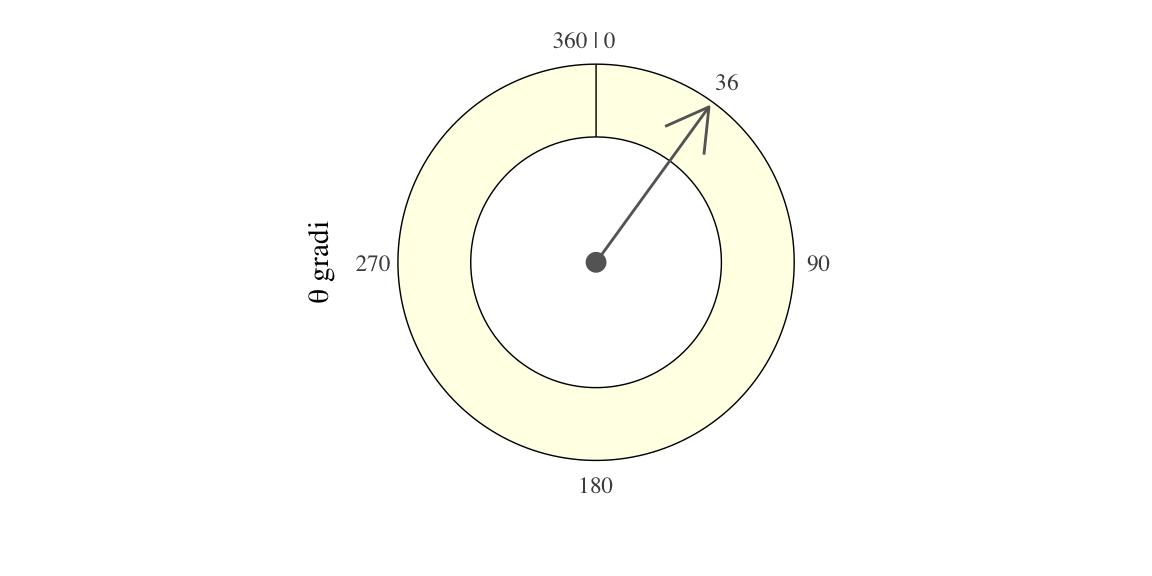
\includegraphics[width=0.8\linewidth]{023_cont_rv_distr_files/figure-latex/unnamed-chunk-1-1} 

}

\caption{Probabilità del numero di successi in $N = 10$ prove bernoulliane indipendenti, ciascuna con una probabilità di successo di 0.90. Il risultato è una distribuzione $\Bin(y \mid 10, 0.9)$. Con solo dieci prove, la distribuzione è fortemente asimmetrica negativa.}\label{fig:unnamed-chunk-1}
\end{figure}

Ma se aumentiamo il numero di prove di un fattore di 100 a
\emph{N} = 1000, senza modificare la probabilità di successo di 0.9, la distribuzione assume una forma campanulare quasi simmetrica. Dunque, de Moivre scoprì che, quando \emph{N} è grande, la funzione Normale (che introdurremo qui sotto), nonostante sia la densità di v.a. continue, fornisce una buona approssimazione alla funzione di massa di probabilità binomiale.

\begin{Shaded}
\begin{Highlighting}[]
\NormalTok{N }\OtherTok{\textless{}{-}} \DecValTok{1000}
\NormalTok{x }\OtherTok{\textless{}{-}} \DecValTok{0}\SpecialCharTok{:}\DecValTok{1000}
\NormalTok{y }\OtherTok{\textless{}{-}} \FunctionTok{dbinom}\NormalTok{(x, N, }\FloatTok{0.9}\NormalTok{)}
\NormalTok{binomial\_limit\_plot }\OtherTok{\textless{}{-}}
  \FunctionTok{tibble}\NormalTok{(}\AttributeTok{x =}\NormalTok{ x, }\AttributeTok{y =}\NormalTok{ y) }\SpecialCharTok{\%\textgreater{}\%}
  \FunctionTok{ggplot}\NormalTok{(}\FunctionTok{aes}\NormalTok{(}\AttributeTok{x =}\NormalTok{ x, }\AttributeTok{y =}\NormalTok{ y)) }\SpecialCharTok{+}
  \FunctionTok{geom\_bar}\NormalTok{(}\AttributeTok{stat =} \StringTok{"identity"}\NormalTok{, }\AttributeTok{color =} \StringTok{"black"}\NormalTok{, }\AttributeTok{size =} \FloatTok{0.2}\NormalTok{) }\SpecialCharTok{+}
  \FunctionTok{xlab}\NormalTok{(}\StringTok{"y"}\NormalTok{) }\SpecialCharTok{+}
  \CommentTok{\# scale\_x\_continuous(breaks = c(0, 2, 4, 6, 8, 1000)) +}
  \FunctionTok{ylab}\NormalTok{(}\StringTok{"Binomial(y | 1000, 0.9)"}\NormalTok{) }\SpecialCharTok{+}
  \FunctionTok{xlim}\NormalTok{(}\DecValTok{850}\NormalTok{, }\DecValTok{950}\NormalTok{)}
\NormalTok{binomial\_limit\_plot}
\end{Highlighting}
\end{Shaded}

\begin{figure}[h]

{\centering 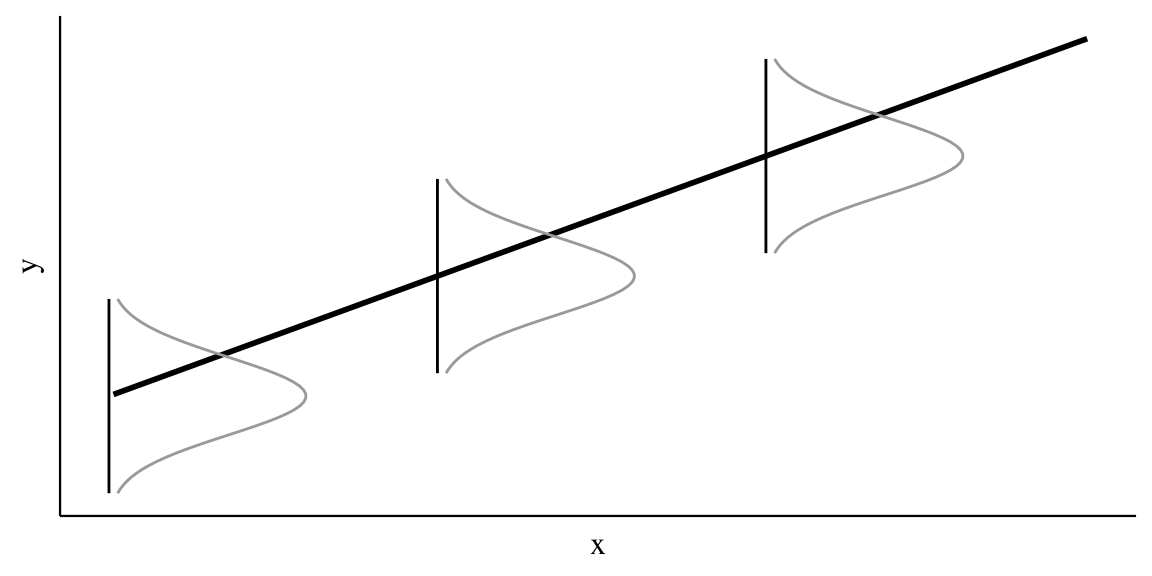
\includegraphics[width=0.8\linewidth]{023_cont_rv_distr_files/figure-latex/unnamed-chunk-2-1} 

}

\caption{Probabilità del numero di successi in $N = 1000$ prove bernoulliane indipendenti, ciascuna con una probabilità di successo di 0.90. Il risultato è una distribuzione $\Bin(y \mid 1000, 0.9)$. Con mille prove, la distribuzione è quasi simmetrica a forma campanulare.}\label{fig:unnamed-chunk-2}
\end{figure}

La distribuzione Normale fu scoperta da Gauss nel 1809 e, storicamente, è intimamente legata al metodo dei minimi quadrati -- si veda l'Appendice \ref{gauss-normale}. Il Paragrafo successivo illustra come si possa giungere alla Normale mediante una simulazione.

\hypertarget{normal-random-walk}{%
\section{La Normale prodotta con una simulazione}\label{normal-random-walk}}

\textcite{McElreath_rethinking} presenta un esempio che illustra come sia possibile giungere alla distribuzione Normale mediante una simulazione. Supponiamo che vi siano mille persone tutte allineate su una linea di partenza. Quando viene dato un segnale, ciascuna persona lancia una moneta e fa un passo in avanti oppure all'indietro a seconda che sia uscita testa o croce. Supponiamo che la lunghezza di ciascun passo vari da 0 a 1 metro. Ciascuna persona lancia una moneta 16 volte e dunque compie 16 passi.

Alla conclusione di queste passeggiate casuali (\emph{random walk}) non possiamo sapere con esattezza dove si troverà ciascuna persona, ma possiamo conoscere con certezza le caratteristiche della distribuzione delle mille distanze dall'origine. Per esempio, possiamo predire in maniera accurata la proporzione di persone che si sono spostate in avanti oppure all'indietro. Oppure, possiamo predire accuratamente la proporzione di persone che si troveranno ad una certa distanza dalla linea di partenza (es., a 1.5 m dall'origine).

Queste predizioni sono possibili perché tali distanze si distribuiscono secondo la legge Normale. È facile simulare questo processo usando \R. I risultati della simulazione sono riportati nella figura \ref{fig:rw-normal-4816}.

\begin{Shaded}
\begin{Highlighting}[]
\FunctionTok{set.seed}\NormalTok{(}\DecValTok{4}\NormalTok{)}
\NormalTok{pos }\OtherTok{\textless{}{-}}
  \FunctionTok{replicate}\NormalTok{(}\DecValTok{100}\NormalTok{, }\FunctionTok{runif}\NormalTok{(}\DecValTok{16}\NormalTok{, }\SpecialCharTok{{-}}\DecValTok{1}\NormalTok{, }\DecValTok{1}\NormalTok{)) }\SpecialCharTok{\%\textgreater{}\%}
  \FunctionTok{as\_tibble}\NormalTok{() }\SpecialCharTok{\%\textgreater{}\%}
  \FunctionTok{rbind}\NormalTok{(}\DecValTok{0}\NormalTok{, .) }\SpecialCharTok{\%\textgreater{}\%}
  \FunctionTok{mutate}\NormalTok{(}\AttributeTok{step =} \DecValTok{0}\SpecialCharTok{:}\DecValTok{16}\NormalTok{) }\SpecialCharTok{\%\textgreater{}\%}
  \FunctionTok{gather}\NormalTok{(key, value, }\SpecialCharTok{{-}}\NormalTok{step) }\SpecialCharTok{\%\textgreater{}\%}
  \FunctionTok{mutate}\NormalTok{(}\AttributeTok{person =} \FunctionTok{rep}\NormalTok{(}\DecValTok{1}\SpecialCharTok{:}\DecValTok{100}\NormalTok{, }\AttributeTok{each =} \DecValTok{17}\NormalTok{)) }\SpecialCharTok{\%\textgreater{}\%}
  \FunctionTok{group\_by}\NormalTok{(person) }\SpecialCharTok{\%\textgreater{}\%}
  \FunctionTok{mutate}\NormalTok{(}\AttributeTok{position =} \FunctionTok{cumsum}\NormalTok{(value)) }\SpecialCharTok{\%\textgreater{}\%}
  \FunctionTok{ungroup}\NormalTok{()}

\FunctionTok{ggplot}\NormalTok{(}
  \AttributeTok{data =}\NormalTok{ pos,}
  \FunctionTok{aes}\NormalTok{(}\AttributeTok{x =}\NormalTok{ step, }\AttributeTok{y =}\NormalTok{ position, }\AttributeTok{group =}\NormalTok{ person)}
\NormalTok{) }\SpecialCharTok{+}
  \FunctionTok{geom\_vline}\NormalTok{(}\AttributeTok{xintercept =} \FunctionTok{c}\NormalTok{(}\DecValTok{4}\NormalTok{, }\DecValTok{8}\NormalTok{, }\DecValTok{16}\NormalTok{), }\AttributeTok{linetype =} \DecValTok{2}\NormalTok{) }\SpecialCharTok{+}
  \FunctionTok{geom\_line}\NormalTok{(}\FunctionTok{aes}\NormalTok{(}\AttributeTok{color =}\NormalTok{ person }\SpecialCharTok{\textless{}} \DecValTok{2}\NormalTok{, }\AttributeTok{alpha =}\NormalTok{ person }\SpecialCharTok{\textless{}} \DecValTok{2}\NormalTok{)) }\SpecialCharTok{+}
  \FunctionTok{scale\_color\_manual}\NormalTok{(}\AttributeTok{values =} \FunctionTok{c}\NormalTok{(}\StringTok{"gray"}\NormalTok{, }\StringTok{"black"}\NormalTok{)) }\SpecialCharTok{+}
  \FunctionTok{scale\_alpha\_manual}\NormalTok{(}\AttributeTok{values =} \FunctionTok{c}\NormalTok{(}\DecValTok{1} \SpecialCharTok{/} \DecValTok{5}\NormalTok{, }\DecValTok{1}\NormalTok{)) }\SpecialCharTok{+}
  \FunctionTok{scale\_x\_continuous}\NormalTok{(}
    \StringTok{"Numero di passi"}\NormalTok{,}
    \AttributeTok{breaks =} \FunctionTok{c}\NormalTok{(}\DecValTok{0}\NormalTok{, }\DecValTok{4}\NormalTok{, }\DecValTok{8}\NormalTok{, }\DecValTok{12}\NormalTok{, }\DecValTok{16}\NormalTok{)}
\NormalTok{  ) }\SpecialCharTok{+}
  \FunctionTok{labs}\NormalTok{(}\AttributeTok{y =} \StringTok{"Posizione"}\NormalTok{) }\SpecialCharTok{+}
  \FunctionTok{theme}\NormalTok{(}\AttributeTok{legend.position =} \StringTok{"none"}\NormalTok{)}
\end{Highlighting}
\end{Shaded}

\begin{figure}[h]

{\centering 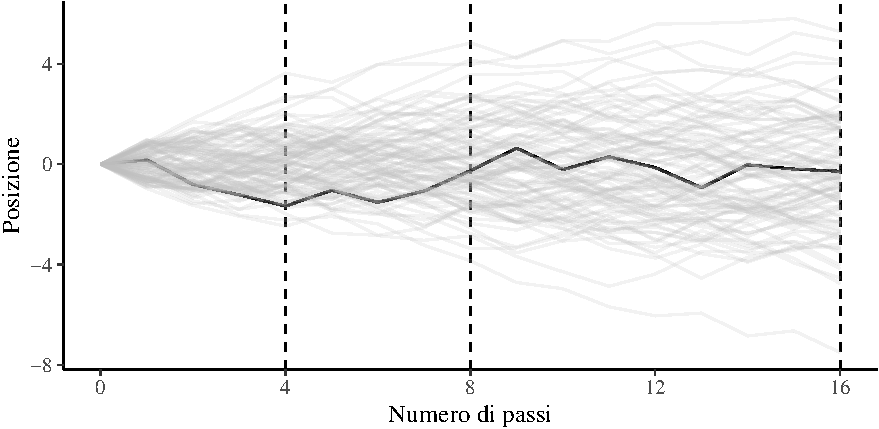
\includegraphics[width=0.8\linewidth]{023_cont_rv_distr_files/figure-latex/rw-normal-4816-1} 

}

\caption{Passeggiata casuale di 4, 8 e 16 passi. La spezzata nera indica la media delle distanze dall'origine come funzione del numero di passi.}\label{fig:rw-normal-4816}
\end{figure}

Un kernel density plot delle distanze ottenute dopo 4, 8 e 16 passi è riportato nella figura \ref{fig:rw-normal-3panels}. Nel pannello di destra, al kernel density plot è stata sovrapposta una densità Normale di opportuni parametri (linea tratteggiata).

\begin{Shaded}
\begin{Highlighting}[]
\NormalTok{p1 }\OtherTok{\textless{}{-}}
\NormalTok{  pos }\SpecialCharTok{\%\textgreater{}\%}
  \FunctionTok{filter}\NormalTok{(step }\SpecialCharTok{==} \DecValTok{4}\NormalTok{) }\SpecialCharTok{\%\textgreater{}\%}
  \FunctionTok{ggplot}\NormalTok{(}\FunctionTok{aes}\NormalTok{(}\AttributeTok{x =}\NormalTok{ position)) }\SpecialCharTok{+}
  \FunctionTok{geom\_line}\NormalTok{(}\AttributeTok{stat =} \StringTok{"density"}\NormalTok{, }\AttributeTok{color =} \StringTok{"black"}\NormalTok{) }\SpecialCharTok{+}
  \FunctionTok{labs}\NormalTok{(}\AttributeTok{title =} \StringTok{"4 passi"}\NormalTok{)}

\NormalTok{p2 }\OtherTok{\textless{}{-}}
\NormalTok{  pos }\SpecialCharTok{\%\textgreater{}\%}
  \FunctionTok{filter}\NormalTok{(step }\SpecialCharTok{==} \DecValTok{8}\NormalTok{) }\SpecialCharTok{\%\textgreater{}\%}
  \FunctionTok{ggplot}\NormalTok{(}\FunctionTok{aes}\NormalTok{(}\AttributeTok{x =}\NormalTok{ position)) }\SpecialCharTok{+}
  \FunctionTok{geom\_density}\NormalTok{(}\AttributeTok{color =} \StringTok{"black"}\NormalTok{, }\AttributeTok{outline.type =} \StringTok{"full"}\NormalTok{) }\SpecialCharTok{+}
  \FunctionTok{labs}\NormalTok{(}\AttributeTok{title =} \StringTok{"8 passi"}\NormalTok{)}

\NormalTok{sd }\OtherTok{\textless{}{-}}
\NormalTok{  pos }\SpecialCharTok{\%\textgreater{}\%}
  \FunctionTok{filter}\NormalTok{(step }\SpecialCharTok{==} \DecValTok{16}\NormalTok{) }\SpecialCharTok{\%\textgreater{}\%}
  \FunctionTok{summarise}\NormalTok{(}\AttributeTok{sd =} \FunctionTok{sd}\NormalTok{(position)) }\SpecialCharTok{\%\textgreater{}\%}
  \FunctionTok{pull}\NormalTok{(sd)}

\NormalTok{p3 }\OtherTok{\textless{}{-}}
\NormalTok{  pos }\SpecialCharTok{\%\textgreater{}\%}
  \FunctionTok{filter}\NormalTok{(step }\SpecialCharTok{==} \DecValTok{16}\NormalTok{) }\SpecialCharTok{\%\textgreater{}\%}
  \FunctionTok{ggplot}\NormalTok{(}\FunctionTok{aes}\NormalTok{(}\AttributeTok{x =}\NormalTok{ position)) }\SpecialCharTok{+}
  \FunctionTok{stat\_function}\NormalTok{(}
    \AttributeTok{fun =}\NormalTok{ dnorm,}
    \AttributeTok{args =} \FunctionTok{list}\NormalTok{(}\AttributeTok{mean =} \DecValTok{0}\NormalTok{, }\AttributeTok{sd =}\NormalTok{ sd),}
    \AttributeTok{linetype =} \DecValTok{2}
\NormalTok{  ) }\SpecialCharTok{+}
  \FunctionTok{geom\_density}\NormalTok{(}\AttributeTok{color =} \StringTok{"black"}\NormalTok{, }\AttributeTok{alpha =} \DecValTok{1} \SpecialCharTok{/} \DecValTok{2}\NormalTok{) }\SpecialCharTok{+}
  \FunctionTok{labs}\NormalTok{(}
    \AttributeTok{title =} \StringTok{"16 passi"}\NormalTok{,}
    \AttributeTok{y =} \StringTok{"Densità"}
\NormalTok{  )}

\NormalTok{(p1 }\SpecialCharTok{|}\NormalTok{ p2 }\SpecialCharTok{|}\NormalTok{ p3) }\SpecialCharTok{\&} \FunctionTok{coord\_cartesian}\NormalTok{(}\AttributeTok{xlim =} \FunctionTok{c}\NormalTok{(}\SpecialCharTok{{-}}\DecValTok{6}\NormalTok{, }\DecValTok{6}\NormalTok{))}
\end{Highlighting}
\end{Shaded}

\begin{figure}[h]

{\centering 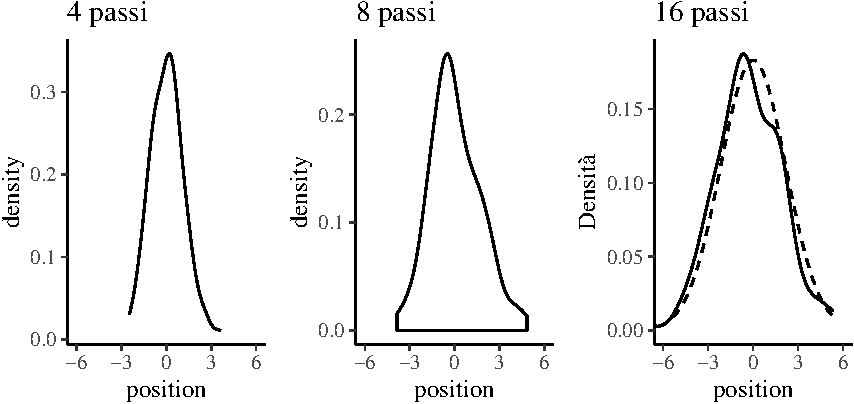
\includegraphics[width=0.8\linewidth]{023_cont_rv_distr_files/figure-latex/rw-normal-3panels-1} 

}

\caption{Kernel density plot dei risultati della passeggiata casuale riportata nella figura precente, dopo 4, 8 e 16 passi. Nel pannello di destra, una densità Normale di opportuni parametri è sovrapposta all'istogramma lisciato.}\label{fig:rw-normal-3panels}
\end{figure}

Questa simulazione mostra che qualunque processo nel quale viene sommato un certo numero di valori casuali, tutti provenienti dalla medesima distribuzione, converge ad una distribuzione Normale. Non importa quale sia la forma della distribuzione di partenza: essa può essere uniforme, come nell'esempio presente, o di qualunque altro tipo. La forma della distribuzione da cui viene realizzato il campionamento determina la velocità della convergenza alla Normale. In alcuni casi la convergenza è lenta; in altri casi la convergenza è molto rapida (come nell'esempio presente).

Da un punto di vista formale, diciamo che una variabile casuale continua \(Y\) ha una distribuzione Normale se la sua densità è

\begin{equation}
f(y; \mu, \sigma) = {1 \over {\sigma\sqrt{2\pi} }} \exp \left\{-\frac{(y -  \mu)^2}{2 \sigma^2} \right\},
\label{eq:normal-formula}
\end{equation}
\noindent
dove \(\mu \in \mathbb{R}\) e \(\sigma > 0\) sono i parametri della distribuzione.

La densità normale è unimodale e simmetrica con una caratteristica forma a campana e con il punto di massima densità in corrispondenza di \(\mu\).

Il significato dei parametri \(\mu\) e \(\sigma\) che appaiono nella \eqref{eq:normal-formula} viene chiarito dalla dimostrazione che

\begin{equation}
\E(X) = \mu, \qquad \Var(X) = \sigma^2.
\end{equation}

\begin{example}

La rappresentazione grafica di quattro densità Normali tutte con media 0 e con deviazioni standard 0.25, 0.5, 1 e 2 è fornita nella figura \ref{fig:gaussian-plot-demo}.

\begin{figure}[h]

{\centering 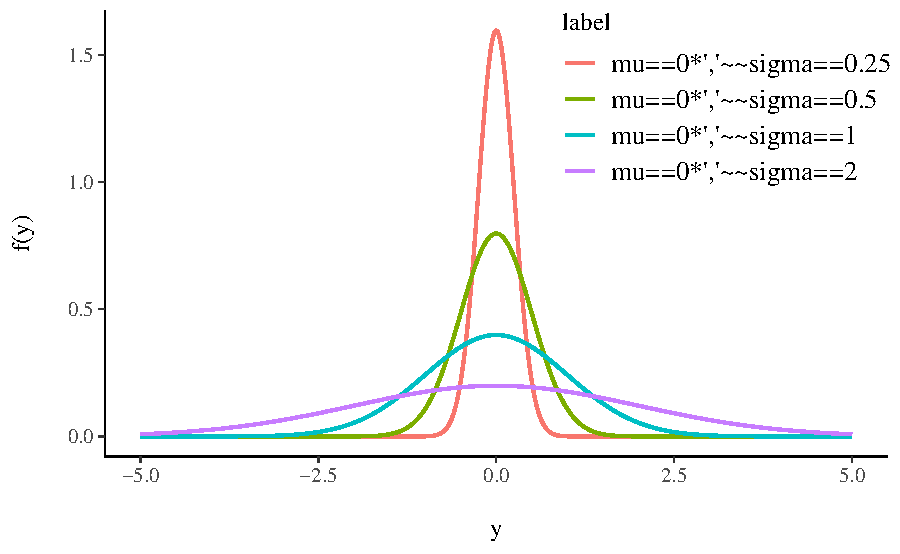
\includegraphics[width=0.8\linewidth]{023_cont_rv_distr_files/figure-latex/gaussian-plot-demo-1} 

}

\caption{Alcune distribuzioni Normali.}\label{fig:gaussian-plot-demo}
\end{figure}

\end{example}

\hypertarget{concentrazione}{%
\subsection{Concentrazione}\label{concentrazione}}

È istruttivo osservare il grado di concentrazione della distribuzione
Normale attorno alla media:

\begin{align}
P(\mu - \sigma < X < \mu + \sigma) &= P (-1 < Z < 1) \simeq 0.683, \notag\\
P(\mu - 2\sigma < X < \mu + 2\sigma) &= P (-2 < Z < 2) \simeq 0.956, \notag\\
P(\mu - 3\sigma < X < \mu + 3\sigma) &= P (-3 < Z < 3) \simeq 0.997. \notag
\end{align}

\noindent
Si noti come un dato la cui distanza dalla media è superiore a 3 volte la deviazione standard presenti un carattere di eccezionalità perché meno del 0.3\% dei dati della distribuzione Normale presentano questa caratteristica.

Per indicare la distribuzione Normale si usa la notazione
\(\mathcal{N}(\mu, \sigma)\).

\hypertarget{funzione-di-ripartizione}{%
\subsection{Funzione di ripartizione}\label{funzione-di-ripartizione}}

Il valore della funzione di ripartizione di \(Y\) nel punto \(y\) è l'area sottesa alla curva di densità \(f(y)\) nella semiretta \((-\infty, y]\). Non esiste alcuna funzione elementare per la funzione di ripartizione

\begin{equation}
F(y) = \int_{-\infty}^y {1 \over {\sigma\sqrt{2\pi} }} \exp \left\{-\frac{(y - \mu)^2}{2\sigma^2} \right\} dy, 
\end{equation}

\noindent
pertanto le probabilità \(P(Y < y)\) vengono calcolate mediante integrazione numerica approssimata. I valori della funzione di ripartizione di una variabile casuale Normale sono dunque forniti da un software.

\begin{example}

Usiamo \R per calcolare la funzione di ripartizione della Normale. La funzione \texttt{pnorm(q,\ mean,\ sd)} restituisce la funzione di ripartizione della Normale con media \texttt{mean} e deviazione standard \texttt{sd}, ovvero l'area sottesa alla funzione di densità di una Normale con media \texttt{mean} e deviazione standard \texttt{sd} nell'intervallo \([-\infty, q]\).

Per esempio, in precedenza abbiamo detto che il 68\% circa dell'area sottesa ad una Normale è compresa nell'intervallo \(\mu \pm \sigma\). Verifichiamo per la distribuzione del QI \(\sim \mathcal{N}(\mu = 100, \sigma = 15)\):

\begin{Shaded}
\begin{Highlighting}[]
\FunctionTok{pnorm}\NormalTok{(}\DecValTok{100} \SpecialCharTok{+} \DecValTok{15}\NormalTok{, }\DecValTok{100}\NormalTok{, }\DecValTok{15}\NormalTok{) }\SpecialCharTok{{-}} \FunctionTok{pnorm}\NormalTok{(}\DecValTok{100} \SpecialCharTok{{-}} \DecValTok{15}\NormalTok{, }\DecValTok{100}\NormalTok{, }\DecValTok{15}\NormalTok{)}
\CommentTok{\#\textgreater{} [1] 0.683}
\end{Highlighting}
\end{Shaded}

\noindent
Il 95\% dell'area è compresa nell'intervallo \(\mu \pm 1.96 \cdot\sigma\):

\begin{Shaded}
\begin{Highlighting}[]
\FunctionTok{pnorm}\NormalTok{(}\DecValTok{100} \SpecialCharTok{+} \FloatTok{1.96} \SpecialCharTok{*} \DecValTok{15}\NormalTok{, }\DecValTok{100}\NormalTok{, }\DecValTok{15}\NormalTok{) }\SpecialCharTok{{-}} \FunctionTok{pnorm}\NormalTok{(}\DecValTok{100} \SpecialCharTok{{-}} \FloatTok{1.96} \SpecialCharTok{*} \DecValTok{15}\NormalTok{, }\DecValTok{100}\NormalTok{, }\DecValTok{15}\NormalTok{)}
\CommentTok{\#\textgreater{} [1] 0.95}
\end{Highlighting}
\end{Shaded}

\noindent
Quasi tutta la distribuzione è compresa nell'intervallo \(\mu \pm 3 \cdot\sigma\):

\begin{Shaded}
\begin{Highlighting}[]
\FunctionTok{pnorm}\NormalTok{(}\DecValTok{100} \SpecialCharTok{+} \DecValTok{3} \SpecialCharTok{*} \DecValTok{15}\NormalTok{, }\DecValTok{100}\NormalTok{, }\DecValTok{15}\NormalTok{) }\SpecialCharTok{{-}} \FunctionTok{pnorm}\NormalTok{(}\DecValTok{100} \SpecialCharTok{{-}} \DecValTok{3} \SpecialCharTok{*} \DecValTok{15}\NormalTok{, }\DecValTok{100}\NormalTok{, }\DecValTok{15}\NormalTok{)}
\CommentTok{\#\textgreater{} [1] 0.997}
\end{Highlighting}
\end{Shaded}

\end{example}

\hypertarget{distribuzione-normale-standard}{%
\subsection{Distribuzione Normale standard}\label{distribuzione-normale-standard}}

La distribuzione Normale di parametri \(\mu = 0\) e \(\sigma = 1\) viene detta \emph{distribuzione Normale standard}. La famiglia Normale è l'insieme avente come elementi tutte le distribuzioni Normali con parametri \(\mu\) e \(\sigma\) diversi. Tutte le distribuzioni Normali si ottengono dalla Normale standard mediante una trasformazione lineare: se \(Y \sim \mathcal{N}(\mu_Y, \sigma_Y)\) allora

\begin{equation}
X = a + b Y \sim \mathcal{N}(\mu_X = a+b \mu_Y, \sigma_X = \left|b\right|\sigma_Y).
\end{equation}

L'area sottesa alla curva di densità di \(\mathcal{N}(\mu, \sigma)\) nella semiretta \((-\infty, y]\) è uguale all'area sottesa alla densità Normale standard nella semiretta \((-\infty, z]\), in cui \(z = (y -\mu_Y )/\sigma_Y\) è il punteggio standard di \(Y\). Per la simmetria della distribuzione, l'area sottesa nella semiretta \([1, \infty)\) è uguale all'area sottesa nella semiretta \((-\infty, 1]\) e quest'ultima coincide con \(F(-1)\). Analogamente, l'area sottesa nell'intervallo \([y_a, y_b]\), con \(y_a < y_b\), è pari a \(F(z_b) - F(z_a)\), dove \(z_a\) e \(z_b\) sono i punteggi standard di \(y_a\) e \(y_b\).

Si ha anche il problema inverso rispetto a quello del calcolo delle aree: dato un numero \(0 \leq p \leq 1\), il problema è quello di determinare un numero \(z \in \mathbb{R}\) tale che \(P(Z < z) = p\). Il valore \(z\) cercato è detto \emph{quantile} di ordine \(p\) della Normale standard e può essere trovato mediante un software.

\begin{example}
Supponiamo che l'altezza degli individui adulti segua la distribuzione Normale di media \(\mu = 1.7\) m e deviazione standard \(\sigma = 0.1\) m. Vogliamo sapere la proporzione di individui adulti con un'altezza compresa tra \(1.7\) e \(1.8\) m.

Il problema ci chiede di trovare l'area sottesa alla distribuzione \(\mathcal{N}(\mu = 1.7, \sigma = 0.1)\) nell'intervallo \([1.7, 1.8]\):

\begin{Shaded}
\begin{Highlighting}[]
\NormalTok{df }\OtherTok{\textless{}{-}} \FunctionTok{tibble}\NormalTok{(}\AttributeTok{x =} \FunctionTok{seq}\NormalTok{(}\FloatTok{1.4}\NormalTok{, }\FloatTok{2.0}\NormalTok{, }\AttributeTok{length.out =} \DecValTok{100}\NormalTok{)) }\SpecialCharTok{\%\textgreater{}\%}
  \FunctionTok{mutate}\NormalTok{(}\AttributeTok{y =} \FunctionTok{dnorm}\NormalTok{(x, }\AttributeTok{mean =} \FloatTok{1.7}\NormalTok{, }\AttributeTok{sd =} \FloatTok{0.1}\NormalTok{))}

\FunctionTok{ggplot}\NormalTok{(df, }\FunctionTok{aes}\NormalTok{(x, y)) }\SpecialCharTok{+}
  \FunctionTok{geom\_area}\NormalTok{(}\AttributeTok{fill =} \StringTok{"sky blue"}\NormalTok{) }\SpecialCharTok{+}
  \FunctionTok{gghighlight}\NormalTok{(x }\SpecialCharTok{\textless{}} \FloatTok{1.8} \SpecialCharTok{\&}\NormalTok{ x }\SpecialCharTok{\textgreater{}} \FloatTok{1.7}\NormalTok{) }\SpecialCharTok{+}
  \FunctionTok{labs}\NormalTok{(}
    \AttributeTok{x =} \StringTok{"Altezza"}\NormalTok{,}
    \AttributeTok{y =} \StringTok{"Densità"}
\NormalTok{  )}
\end{Highlighting}
\end{Shaded}

\begin{center}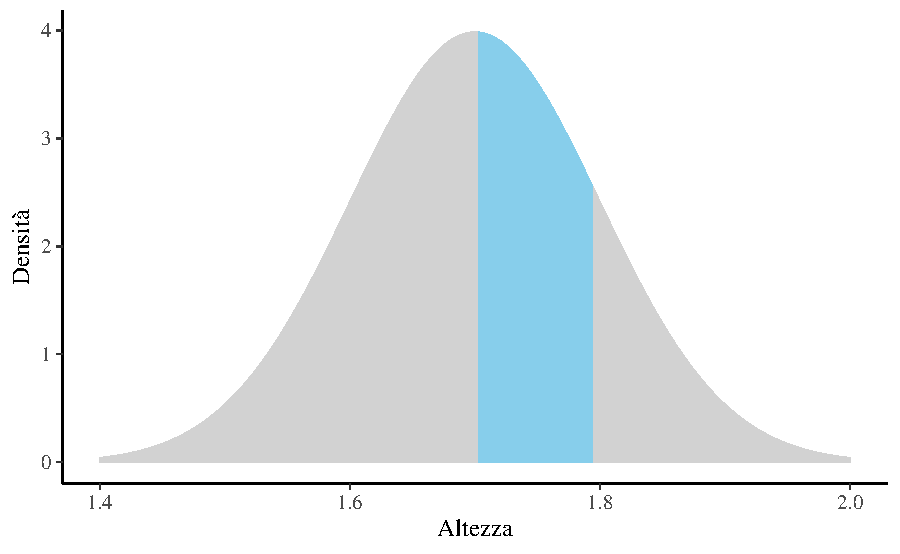
\includegraphics[width=0.8\linewidth]{023_cont_rv_distr_files/figure-latex/unnamed-chunk-6-1} \end{center}

\noindent
La risposta si trova utilizzando la funzione di
ripartizione \(F(X)\) della legge \(\mathcal{N}(1.7, 0.1)\) in
corrispondenza dei due valori forniti dal problema:
\(F(X = 1.8) - F(X = 1.7)\). Utilizzando la seguente istruzione

\begin{Shaded}
\begin{Highlighting}[]
\FunctionTok{pnorm}\NormalTok{(}\FloatTok{1.8}\NormalTok{, }\FloatTok{1.7}\NormalTok{, }\FloatTok{0.1}\NormalTok{) }\SpecialCharTok{{-}} \FunctionTok{pnorm}\NormalTok{(}\FloatTok{1.7}\NormalTok{, }\FloatTok{1.7}\NormalTok{, }\FloatTok{0.1}\NormalTok{)}
\CommentTok{\#\textgreater{} [1] 0.341}
\end{Highlighting}
\end{Shaded}

\noindent
otteniamo il \(31.43\%\).

In maniera equivalente, possiamo standardizzare i valori che delimitano l'intervallo considerato e utilizzare la funzione di ripartizione della normale standardizzata. I limiti inferiore e superiore dell'intervallo sono

\[
z_{\text{inf}} = \frac{1.7 - 1.7}{0.1} = 0, \quad z_{\text{sup}} = \frac{1.8 - 1.7}{0.1} = 1.0,
\]

\noindent 
quindi otteniamo

\begin{Shaded}
\begin{Highlighting}[]
\FunctionTok{pnorm}\NormalTok{(}\FloatTok{1.0}\NormalTok{, }\DecValTok{0}\NormalTok{, }\DecValTok{1}\NormalTok{) }\SpecialCharTok{{-}} \FunctionTok{pnorm}\NormalTok{(}\DecValTok{0}\NormalTok{, }\DecValTok{0}\NormalTok{, }\DecValTok{1}\NormalTok{)}
\CommentTok{\#\textgreater{} [1] 0.341}
\end{Highlighting}
\end{Shaded}

Il modo più semplice per risolvere questo problema resta comunque quello di rendersi conto che la probabilità richiesta non è altro che la metà dell'area sottesa dalle distribuzioni Normali nell'intervallo \([\mu - \sigma, \mu + \sigma]\), ovvero \(0.683/2\).
\end{example}

\hypertarget{funzione-di-ripartizione-della-variabile-casuale-normale-standard-e-funzione-logistica}{%
\subsubsection{Funzione di ripartizione della variabile casuale normale standard e funzione logistica}\label{funzione-di-ripartizione-della-variabile-casuale-normale-standard-e-funzione-logistica}}

Si noti che la funzione logistica (in blu), pur essendo del tutto diversa dalla Normale dal punto di vista formale, assomiglia molto alla Normale standard quando le due cdf hanno la stessa varianza.

\begin{Shaded}
\begin{Highlighting}[]
\FunctionTok{tibble}\NormalTok{(}\AttributeTok{x =} \FunctionTok{c}\NormalTok{(}\SpecialCharTok{{-}}\DecValTok{3}\NormalTok{, }\DecValTok{3}\NormalTok{)) }\SpecialCharTok{\%\textgreater{}\%}
  \FunctionTok{ggplot}\NormalTok{(}\FunctionTok{aes}\NormalTok{(}\AttributeTok{x =}\NormalTok{ x)) }\SpecialCharTok{+}
  \FunctionTok{stat\_function}\NormalTok{(}\AttributeTok{fun =}\NormalTok{ pnorm) }\SpecialCharTok{+}
  \FunctionTok{stat\_function}\NormalTok{(}
    \AttributeTok{fun =}\NormalTok{ plogis,}
    \AttributeTok{args =} \FunctionTok{list}\NormalTok{(}\AttributeTok{scale =} \FloatTok{0.56}\NormalTok{),}
    \AttributeTok{col =} \StringTok{"sky blue"}
\NormalTok{  )}
\end{Highlighting}
\end{Shaded}

\begin{center}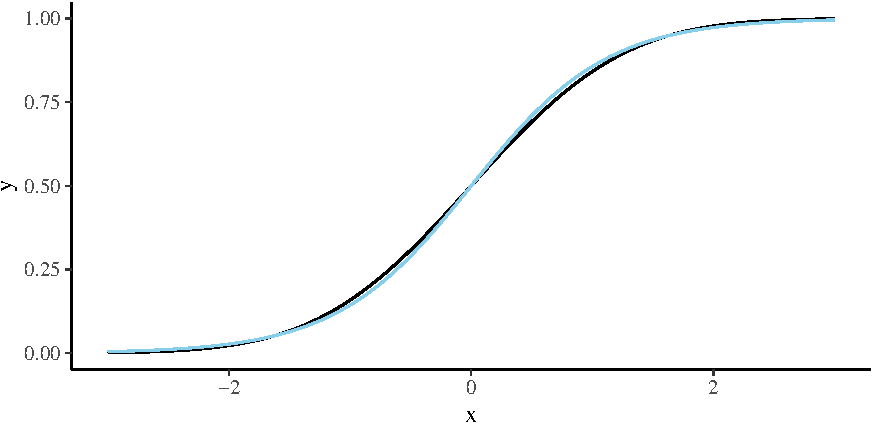
\includegraphics[width=0.8\linewidth]{023_cont_rv_distr_files/figure-latex/unnamed-chunk-9-1} \end{center}

\hypertarget{teorema-del-limite-centrale}{%
\section{Teorema del limite centrale}\label{teorema-del-limite-centrale}}

Laplace dimostrò il teorema del limite centrale (TLC) nel 1812. Il TLC ci dice che se prendiamo una sequenza di variabili casuali indipendenti e le sommiamo, tale somma tende a distribuirisi come una Normale. Il TLC specifica inoltre, sulla base dei valori attesi e delle varianze delle v.c. che vengono sommate, quali saranno i parametri della distribuzione Normale così ottenuta.

\begin{theorem}
Si supponga che \(Y = Y_1, Y_2, \ldots, Y_N\) sia una sequenza di v.a. i.i.d. con \(\E(Y_n) = \mu\) e \(\SD(Y_n) = \sigma\). Si definisca una nuova v.c. come la media di \(Y\):

\[
Z = \frac{1}{N} \sum_{n=1}^N Y_n.
\]
\noindent
Con \(N \rightarrow \infty\), \(Z\) tenderà ad una Normale con lo stesso valore atteso di \(Y_n\) e una deviazione standard che sarà più piccola della deviazione standard originaria di un fattore pari a \(\sqrt{\frac{1}{\sqrt{N}}}\):

\begin{equation}
p_Z(z) \rightarrow \mathcal{N}\left(z \ \Bigg| \ \mu, \, \frac{1}{\sqrt{N}} \cdot \sigma \right).
\end{equation}
\end{theorem}

Il TLC può essere generalizzato a variabili che non hanno la stessa distribuzione purché siano indipendenti e abbiano aspettative e varianze finite.

Molti fenomeni naturali, come l'altezza dell'uomo adulto di entrambi i sessi, sono il risultato di una serie di effetti additivi relativamente piccoli, la cui combinazione porta alla normalità, indipendentemente da come gli effetti additivi sono distribuiti. In pratica, questo è il motivo per cui la distribuzione normale ha senso come rappresentazione di molti fenomeni naturali.

\hypertarget{distribuzione-chi-quadrato}{%
\section{Distribuzione Chi-quadrato}\label{distribuzione-chi-quadrato}}

Dalla Normale deriva la distribuzione \(\chi^2\). La distribuzione \(\chi^2_{~k}\) con \(k\) gradi di libertà descrive la variabile casuale

\[
Z_1^2 + Z_2^2 + \dots + Z_k^2,
\]
\noindent
dove \(Z_1, Z_2, \dots, Z_k\) sono variabili casuali i.i.d. con distribuzione Normale standard \(\mathcal{N}(0, 1)\). La variabile casuale chi-quadrato dipende dal parametro intero positivo \(\nu = k\) che ne identifica il numero di gradi di libertà. La densità di probabilità di \(\chi^2_{~\nu}\) è

\[
f(x) = C_{\nu} x^{\nu/2-1} \exp (-x/2), \qquad \text{se } x > 0,
\]
\noindent
dove \(C_{\nu}\) è una costante positiva.

\hypertarget{proprietuxe0}{%
\subsection{Proprietà}\label{proprietuxe0}}

\begin{itemize}
\tightlist
\item
  La distribuzione di densità \(\chi^2_{~\nu}\) è asimmetrica.
\item
  Il valore atteso di una variabile \(\chi^2_{~\nu}\) è uguale a \(\nu\).
\item
  La varianza di una variabile \(\chi^2_{~\nu}\) è uguale a \(2\nu\).
\item
  Per \(k \rightarrow \infty\), la \(\chi^2_{~\nu} \rightarrow \mathcal{N}\).
\item
  Se \(X\) e \(Y\) sono due variabili casuali chi-quadrato indipendenti con \(\nu_1\) e \(\nu_2\) gradi di libertà, ne segue che \(X + Y \sim \chi^2_m\), con \(m = \nu_1 + \nu_2\). Tale principio si estende a qualunque numero finito di variabili casuali chi-quadrato indipendenti.
\end{itemize}

\begin{example}

Usiamo \(\R\) per disegnare la densità chi-quadrato con 3 gradi di libertà dividendo l'area sottesa alla curva di densità in due parti uguali.

\begin{Shaded}
\begin{Highlighting}[]
\NormalTok{df }\OtherTok{\textless{}{-}} \FunctionTok{tibble}\NormalTok{(}\AttributeTok{x =} \FunctionTok{seq}\NormalTok{(}\DecValTok{0}\NormalTok{, }\FloatTok{15.0}\NormalTok{, }\AttributeTok{length.out =} \DecValTok{100}\NormalTok{)) }\SpecialCharTok{\%\textgreater{}\%}
  \FunctionTok{mutate}\NormalTok{(}\AttributeTok{y =} \FunctionTok{dchisq}\NormalTok{(x, }\DecValTok{3}\NormalTok{))}

\FunctionTok{ggplot}\NormalTok{(df, }\FunctionTok{aes}\NormalTok{(x, y)) }\SpecialCharTok{+}
  \FunctionTok{geom\_area}\NormalTok{(}\AttributeTok{fill =} \StringTok{"sky blue"}\NormalTok{) }\SpecialCharTok{+}
  \FunctionTok{gghighlight}\NormalTok{(x }\SpecialCharTok{\textless{}} \DecValTok{3}\NormalTok{) }\SpecialCharTok{+}
  \FunctionTok{labs}\NormalTok{(}
    \AttributeTok{x =} \StringTok{"V.a. chi{-}quadrato con 3 gradi di libertà"}\NormalTok{,}
    \AttributeTok{y =} \StringTok{"Densità"}
\NormalTok{  )}
\end{Highlighting}
\end{Shaded}

\begin{center}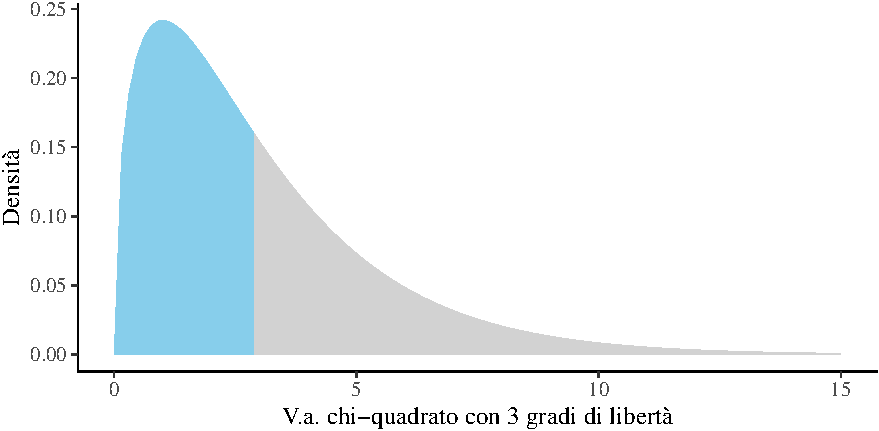
\includegraphics[width=0.8\linewidth]{023_cont_rv_distr_files/figure-latex/unnamed-chunk-10-1} \end{center}

\end{example}

\begin{example}

La figura \ref{fig:alcune-chi-quadrato} mostra alcune distribuzioni Chi-quadrato variando il parametro \(\nu\).

\begin{figure}[h]

{\centering 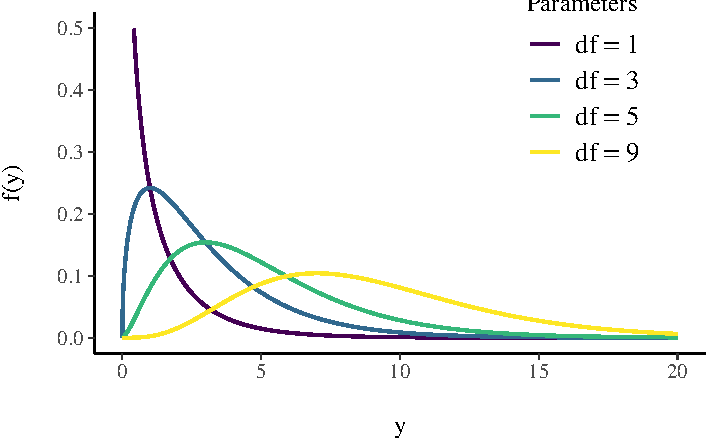
\includegraphics[width=0.8\linewidth]{023_cont_rv_distr_files/figure-latex/alcune-chi-quadrato-1} 

}

\caption{Alcune distribuzioni Chi-quadrato.}\label{fig:alcune-chi-quadrato}
\end{figure}

\end{example}

\hypertarget{distribuzione-t-di-student}{%
\section{\texorpdfstring{Distribuzione \(t\) di Student}{Distribuzione t di Student}}\label{distribuzione-t-di-student}}

Dalle distribuzioni Normale e Chi quadrato deriva un'altra distribuzione molto nota, la \(t\) di Student. Se \(Z \sim \mathcal{N}\) e \(W \sim \chi^2_{~\nu}\) sono due variabili casuali indipendenti, allora il rapporto

\begin{equation}
T = \frac{Z}{\Big( \frac{W}{\nu}\Big)^{\frac{1}{2}}}
\end{equation}
\noindent
definisce la distribuzione \(t\) di Student con \(\nu\) gradi di libertà. Si usa scrivere \(T \sim t_{\nu}\). L'andamento della distribuzione \(t\) di Student è simile a quello della distribuzione Normale, ma ha una maggiore dispersione (ha le code più pesanti di una Normale, ovvero ha una varianza maggiore di 1).

\hypertarget{proprietuxe0-1}{%
\subsection{Proprietà}\label{proprietuxe0-1}}

La variabile casuale \(t\) di Student soddisfa le seguenti proprietà:

\begin{enumerate}
\def\labelenumi{\arabic{enumi}.}
\item
  Per \(\nu \rightarrow \infty\), \(t_{\nu}\) tende alla normale standard
  \(\mathcal{N}(0, 1)\).
\item
  La densità della \(t_{\nu}\) è una funzione simmetrica con valore
  atteso nullo.
\item
  Per \(\nu > 2\), la varianza della \(t_{\nu}\) vale \(\nu/(\nu - 2)\);
  pertanto è sempre maggiore di 1 e tende a 1 per
  \(\nu \rightarrow \infty\).
\end{enumerate}

\begin{example}

La figura \ref{fig:alcune-t-student} mostra alcune distribuzioni \(t\) di Student variando il parametro \(\nu\).

\begin{figure}[h]

{\centering 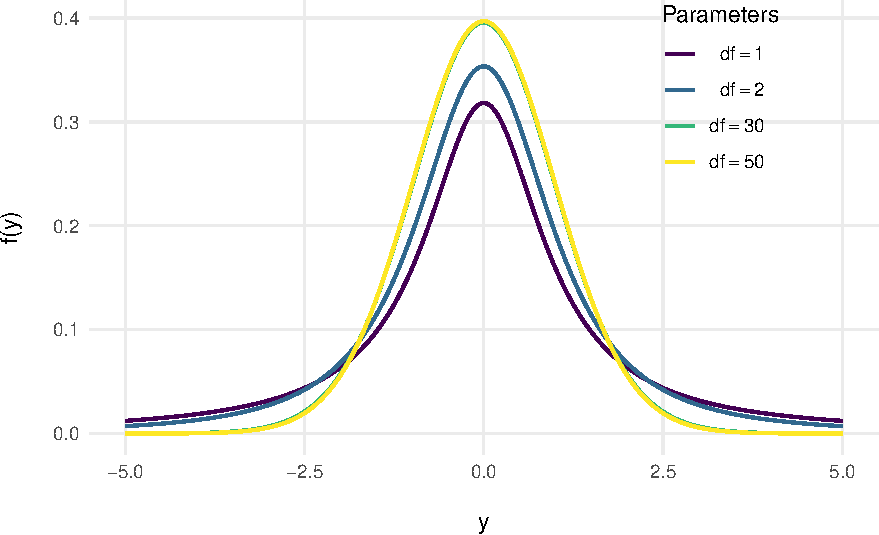
\includegraphics[width=0.8\linewidth]{023_cont_rv_distr_files/figure-latex/alcune-t-student-1} 

}

\caption{Alcune distribuzioni $t$ di Student.}\label{fig:alcune-t-student}
\end{figure}

\end{example}

\hypertarget{funzione-beta-di-eulero}{%
\section{Funzione beta di Eulero}\label{funzione-beta-di-eulero}}

La funzione beta di Eulero è una funzione matematica, \emph{non} una densità di probabilità. La menzioniamo qui perché viene utilizzata nella distribuzione Beta. La funzione beta si può scrivere in molti modi; per i nostri scopi, può essere scritta nel modo seguente:
\begin{equation}
B(\alpha, \beta) = \frac{\Gamma(\alpha)\Gamma(\beta)}{\Gamma(\alpha + \beta)}\,,
\end{equation}
\noindent
dove \(\Gamma(x)\) è la funzione Gamma, ovvero il fattoriale discendente, cioè
\begin{equation}
x(x-1)(x-2)\ldots (x-n+1)\notag\,.
\end{equation}

\hypertarget{distribuzione-beta}{%
\section{Distribuzione Beta}\label{distribuzione-beta}}

Una distribuzione che viene usata per modellare percentuali e proporzioni è la distribuzione Beta in quanto è definita sull'intervallo \((0; 1)\) -- ma non include i valori 0 o 1. La distribuzione Beta è una distribuzione estremamente flessibile e può assumere molti tipi di forme diverse (un'illustrazione è fornita dalla seguente \href{https://en.wikipedia.org/wiki/File:PDF_of_the_Beta_distribution.gif}{GIF animata}). Una definizione formale è la seguente.

\begin{definition}
Sia \(\pi\) una variabile casuale che può assumere qualsiasi valore compreso tra 0 e 1, cioè \(\pi \in [0, 1]\). Diremo che \(\pi\) segue la distribuzione Beta di parametri \(\alpha\) e \(\beta\), \(\pi \sim \text{Beta}(\alpha, \beta)\), se la sua densità è
\begin{align}
\text{Beta}(\pi \mid \alpha, \beta) &= \frac{1}{B(\alpha, \beta)}\pi^{\alpha-1} (1-\pi)^{\beta-1}\notag\\ 
&=  \frac{\Gamma(\alpha+ \beta)}{\Gamma(\alpha)\Gamma(\beta)}\pi^{\alpha-1} (1-\pi)^{\beta-1} \quad \text{per } \pi \in [0, 1]\,,
\label{eq:beta-distr-formula}
\end{align}
laddove \(B(\alpha, \beta)\) è la funzione beta.
\end{definition}

I termini \(\alpha\) e \(\beta\) sono i parametri della distribuzione Beta e devono essere entrambi positivi. Tali parametri possono essere interpretati come l'espressione delle nostre credenze a priori relativamente alla probabilità di successo. Il parametro \(\alpha\) rappresenta il numero di ``successi'' e il parametro \(\beta\) il numero di ``insuccessi'':
\begin{equation}
\frac{\text{Numero di successi}}{\text{Numero di successi} + \text{Numero di insuccessi}} = \frac{\alpha}{\alpha + \beta}\notag\,.
\end{equation}

Il rapporto \(\frac{1}{B(\alpha, \beta)} = \frac{\Gamma(\alpha+b)}{\Gamma(\alpha)\Gamma(\beta)}\) è una costante di normalizzazione:
\begin{equation}
\int_0^1 \pi^{\alpha-1} (1-\pi)^{\beta-1} = \frac{\Gamma(\alpha+b)}{\Gamma(\alpha)\Gamma(\beta)}\,.
\end{equation}

Il valore atteso, la moda e la varianza di una distribuzione Beta sono dati dalle seguenti equazioni:
\begin{equation}
\E(\pi) = \frac{\alpha}{\alpha+\beta}\,,
\label{eq:beta-mean}
\end{equation}

\begin{equation}
\Mo(\pi) = \frac{\alpha-1}{\alpha+\beta-2}\,,
\label{eq:beta-mode}
\end{equation}

\begin{equation}
\Var(\pi) = \frac{\alpha \beta}{(\alpha+\beta)^2 (\alpha+\beta+1)}\,.
\label{eq:beta-var}
\end{equation}

\emph{Attenzione alle parole.} In questo contesto, il termine ``beta'' viene utilizzato con tre significati diversi:

\begin{itemize}
\tightlist
\item
  la distribuzione di densità Beta,
\item
  la funzione matematica beta,
\item
  il parametro \(\beta\).
\end{itemize}

\begin{example}

Al variare di \(\alpha\) e \(\beta\) si ottengono molte distribuzioni di forma diversa; per \(\alpha = \beta = 1\) si ha la densità uniforme. Vari esempi di distribuzioni Beta sono mostrati nella figura \ref{fig:some-beta-distr}.

\begin{figure}[h]

{\centering 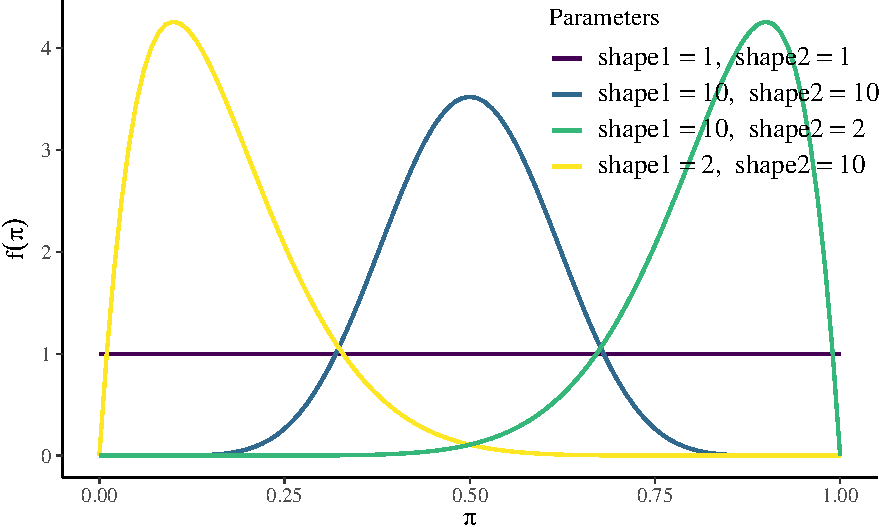
\includegraphics[width=0.8\linewidth]{023_cont_rv_distr_files/figure-latex/some-beta-distr-1} 

}

\caption{Alcune distribuzioni Beta.}\label{fig:some-beta-distr}
\end{figure}

\end{example}

\begin{example}
\protect\hypertarget{exm:beta-tuning}{}\label{exm:beta-tuning}Nel disturbo depressivo la recidiva è definita come la comparsa di un nuovo episodio depressivo che si manifesta dopo un prolungato periodo di recupero (6-12 mesi) con stato di eutimia (umore relativamente normale). Supponiamo che una serie di studi mostri una comparsa di recidiva in una proporzione che va dal 20\% al 60\% dei casi, con una media del 40\% \autocite[per una recente discussione, si veda][]{nuggerud2020analysis}. Sulla base di queste ipotetiche informazioni, è possibile usare la distribuzione Beta per rappresentare le nostre credenze a priori relativamente alla probabilità di recidiva. Per fare questo dobbiamo trovare i parametri della distribuzione Beta tali per cui la massa della densità sia compresa tra 0.2 e 0.6, con la media in corrispondenza di 0.4. Procedendo per tentativi ed errori, ed usando la funzione \texttt{bayesrules::plot\_beta()}, un risultato possibile è \(\Beta(16, 24)\).

\begin{Shaded}
\begin{Highlighting}[]
\NormalTok{find\_pars }\OtherTok{\textless{}{-}} \ControlFlowTok{function}\NormalTok{(ev, n) \{}
\NormalTok{  a }\OtherTok{\textless{}{-}}\NormalTok{ ev }\SpecialCharTok{*}\NormalTok{ n}
\NormalTok{  b }\OtherTok{\textless{}{-}}\NormalTok{ n }\SpecialCharTok{{-}}\NormalTok{ a}
  \FunctionTok{return}\NormalTok{(}\FunctionTok{c}\NormalTok{(}\FunctionTok{round}\NormalTok{(a), }\FunctionTok{round}\NormalTok{(b)))}
\NormalTok{\}}

\NormalTok{pars }\OtherTok{\textless{}{-}} \FunctionTok{find\_pars}\NormalTok{(.}\DecValTok{4}\NormalTok{, }\DecValTok{40}\NormalTok{)}
\NormalTok{pars}
\CommentTok{\#\textgreater{} [1] 16 24}
\NormalTok{bayesrules}\SpecialCharTok{::}\FunctionTok{plot\_beta}\NormalTok{(pars[}\DecValTok{1}\NormalTok{], pars[}\DecValTok{2}\NormalTok{])}
\end{Highlighting}
\end{Shaded}

\begin{center}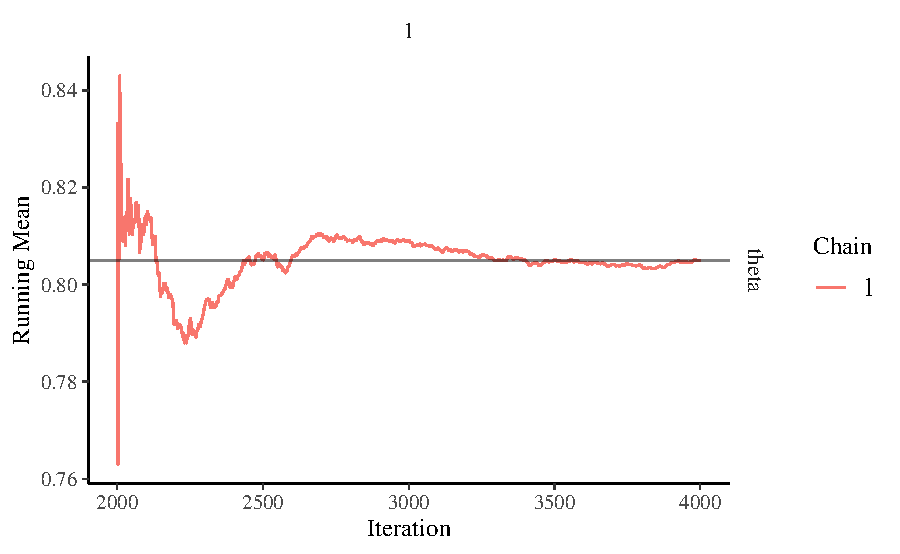
\includegraphics[width=0.8\linewidth]{023_cont_rv_distr_files/figure-latex/unnamed-chunk-11-1} \end{center}

La media della distribuzione a priori diventa:

\begin{Shaded}
\begin{Highlighting}[]
\DecValTok{16} \SpecialCharTok{/}\NormalTok{ (}\DecValTok{16} \SpecialCharTok{+} \DecValTok{24}\NormalTok{)}
\CommentTok{\#\textgreater{} [1] 0.4}
\end{Highlighting}
\end{Shaded}

\noindent
e la moda è

\begin{Shaded}
\begin{Highlighting}[]
\NormalTok{(}\DecValTok{16} \SpecialCharTok{{-}} \DecValTok{1}\NormalTok{) }\SpecialCharTok{/}\NormalTok{ (}\DecValTok{16} \SpecialCharTok{+} \DecValTok{24} \SpecialCharTok{{-}} \DecValTok{2}\NormalTok{)}
\CommentTok{\#\textgreater{} [1] 0.395}
\end{Highlighting}
\end{Shaded}

\noindent
Inoltre, la deviazione standard della distribuzione a priori diventa

\begin{Shaded}
\begin{Highlighting}[]
\FunctionTok{sqrt}\NormalTok{((}\DecValTok{16} \SpecialCharTok{*} \DecValTok{24}\NormalTok{) }\SpecialCharTok{/}\NormalTok{ ((}\DecValTok{16} \SpecialCharTok{+} \DecValTok{24}\NormalTok{)}\SpecialCharTok{\^{}}\DecValTok{2} \SpecialCharTok{*}\NormalTok{ (}\DecValTok{16} \SpecialCharTok{+} \DecValTok{24} \SpecialCharTok{+} \DecValTok{1}\NormalTok{)))}
\CommentTok{\#\textgreater{} [1] 0.0765}
\end{Highlighting}
\end{Shaded}

\noindent
uguale a circa 8 punti percentuali. Questo significa che le nostre credenze a priori rispetto la possibilità di recidiva tendono a deviare di circa 8 punti percentuali rispetto alla media della distribuzione a priori del 40\%.
\end{example}

\hypertarget{distribuzione-di-cauchy}{%
\section{Distribuzione di Cauchy}\label{distribuzione-di-cauchy}}

La distribuzione di Cauchy è un caso speciale della distribuzione di \(t\) di Student con 1 grado di libertà. È definita da una densità di probabilità che corrisponde alla funzione, dipendente da due parametri \(\theta\) e \(d\) (con la condizione \(d > 0\)),

\begin{equation}
f(x; \theta, d) = \frac{1}{\pi d} \frac{1}{1 + \left(\frac{x - \theta}{d} \right)^2},
\end{equation}
dove \(\theta\) è la mediana della distribuzione e \(d\) ne misura la larghezza a metà altezza.

\hypertarget{distribuzione-log-normale}{%
\section{Distribuzione log-normale}\label{distribuzione-log-normale}}

Sia \(y\) una variabile casuale avente distribuzione normale con media \(\mu\) e varianza \(\sigma^2\). Definiamo poi una nuova variabile casuale \(x\) attraverso la relazione
\[
x = e^y \quad \Longleftrightarrow \quad y = \log x.
\]
Il dominio di definizione della \(x\) è il semiasse \(x > 0\) e la densità di probabilità \(f(x)\) è data da
\begin{equation}
f(x) = \frac{1}{\sigma \sqrt{2 \pi}} \frac{1}{x} \exp \left\{-\frac{(\log x -  \mu)^2}{2 \sigma^2} \right\}.
\end{equation}
\noindent
Questa funzione di densità si chiama log-normale.

Il valore atteso e la varianza di una distribuzione log-normale sono dati dalle seguenti equazioni:
\begin{equation}
\E(x) = \exp \left\{\mu + \frac{\sigma^2}{2} \right\}.
\end{equation}

\begin{equation}
\Var(x) = \exp \left\{2 \mu + \sigma^2 \right\} \left(\exp \left\{\sigma^2 \right\}  -1\right).
\end{equation}

Si può dimostrare che il prodotto di variabili casuali log-normali ed indipendenti segue una distribuzione log-normale.

\hypertarget{distribuzione-di-pareto}{%
\section{Distribuzione di Pareto}\label{distribuzione-di-pareto}}

La distribuzione paretiana (o distribuzione di Pareto) è una distribuzione di probabilità continua e così chiamata in onore di Vilfredo Pareto. La distribuzione di Pareto è una distribuzione di probabilità con legge di potenza utilizzata nella descrizione di fenomeni sociali e molti altri tipi di fenomeni osservabili. Originariamente applicata per descrivere la distribuzione del reddito in una società, adattandosi alla tendenza che una grande porzione di ricchezza è detenuta da una piccola frazione della popolazione, la distribuzione di Pareto è diventata colloquialmente nota e indicata come il principio di Pareto, o ``regola 80-20''. Questa regola afferma che, ad esempio, l'80\% della ricchezza di una società è detenuto dal 20\% della sua popolazione. Viene spesso applicata nello studio della distribuzione del reddito, della dimensione dell'impresa, della dimensione di una popolazione e nelle fluttuazioni del prezzo delle azioni.

La densità di una distribuzione di Pareto é

\[
f(x)=(x_m/x)^\alpha,
\]
\noindent
dove \(x_m\) (parametro di scala) è il minimo (necessariamente positivo) valore possibile di \(X\) e \(\alpha\) è un parametro di forma.

\begin{Shaded}
\begin{Highlighting}[]
\NormalTok{x }\OtherTok{\textless{}{-}} \FunctionTok{seq}\NormalTok{(}\DecValTok{1}\NormalTok{, }\DecValTok{5}\NormalTok{, }\FloatTok{0.05}\NormalTok{)}
\NormalTok{a3 }\OtherTok{\textless{}{-}} \DecValTok{3} \SpecialCharTok{/}\NormalTok{ x}\SpecialCharTok{\^{}}\NormalTok{(}\DecValTok{4}\NormalTok{)}
\NormalTok{a2 }\OtherTok{\textless{}{-}} \DecValTok{2} \SpecialCharTok{/}\NormalTok{ x}\SpecialCharTok{\^{}}\NormalTok{(}\DecValTok{3}\NormalTok{)}
\NormalTok{a1 }\OtherTok{\textless{}{-}} \DecValTok{1} \SpecialCharTok{/}\NormalTok{ x}\SpecialCharTok{\^{}}\NormalTok{(}\DecValTok{2}\NormalTok{)}
\NormalTok{df }\OtherTok{\textless{}{-}} \FunctionTok{bind\_rows}\NormalTok{(}
  \FunctionTok{tibble}\NormalTok{(}\AttributeTok{x =}\NormalTok{ x, }\AttributeTok{p =}\NormalTok{ a3, }\AttributeTok{alpha =} \StringTok{"3"}\NormalTok{),}
  \FunctionTok{tibble}\NormalTok{(}\AttributeTok{x =}\NormalTok{ x, }\AttributeTok{p =}\NormalTok{ a2, }\AttributeTok{alpha =} \StringTok{"2"}\NormalTok{),}
  \FunctionTok{tibble}\NormalTok{(}\AttributeTok{x =}\NormalTok{ x, }\AttributeTok{p =}\NormalTok{ a1, }\AttributeTok{alpha =} \StringTok{"1"}\NormalTok{)}
\NormalTok{)}
\NormalTok{gg }\OtherTok{\textless{}{-}}\NormalTok{ df }\SpecialCharTok{\%\textgreater{}\%}
  \FunctionTok{ggplot}\NormalTok{(}\FunctionTok{aes}\NormalTok{(}\AttributeTok{x =}\NormalTok{ x, }\AttributeTok{y =}\NormalTok{ p, }\AttributeTok{group =}\NormalTok{ alpha)) }\SpecialCharTok{+}
  \FunctionTok{geom\_line}\NormalTok{(}\FunctionTok{aes}\NormalTok{(}\AttributeTok{color =}\NormalTok{ alpha)) }\SpecialCharTok{+}
  \FunctionTok{xlim}\NormalTok{(}\DecValTok{1}\NormalTok{, }\DecValTok{5}\NormalTok{) }\SpecialCharTok{+}
  \FunctionTok{ggtitle}\NormalTok{(}\StringTok{"Densità di Pareto per alcuni valori del parametro di forma"}\NormalTok{) }\SpecialCharTok{+}
  \FunctionTok{ylab}\NormalTok{(}\StringTok{"P(X = x)"}\NormalTok{) }\SpecialCharTok{+}
  \FunctionTok{scale\_colour\_viridis}\NormalTok{(}
    \AttributeTok{discrete =} \ConstantTok{TRUE}\NormalTok{, }\AttributeTok{labels =} \FunctionTok{parse\_format}\NormalTok{()}
\NormalTok{  ) }\SpecialCharTok{+}
  \FunctionTok{labs}\NormalTok{(}
    \AttributeTok{x =} \StringTok{"}\SpecialCharTok{\textbackslash{}n}\StringTok{y"}\NormalTok{,}
    \AttributeTok{y =} \StringTok{"f(y)}\SpecialCharTok{\textbackslash{}n}\StringTok{"}
\NormalTok{  )}
\FunctionTok{print}\NormalTok{(gg)}
\end{Highlighting}
\end{Shaded}

\begin{center}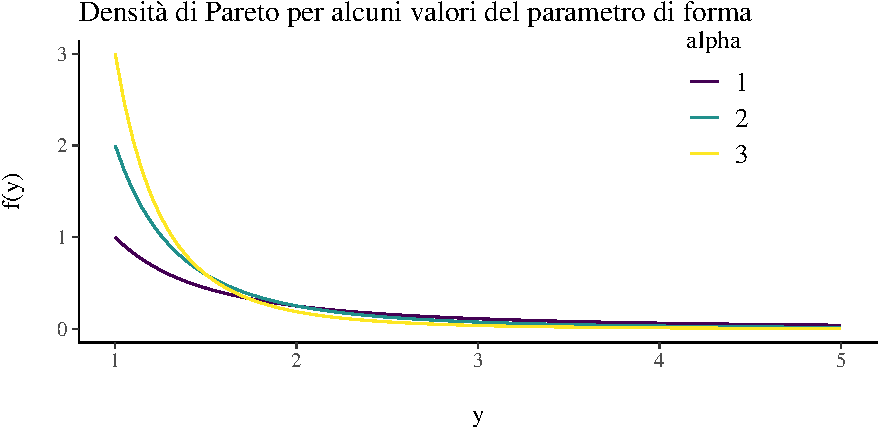
\includegraphics[width=0.8\linewidth]{023_cont_rv_distr_files/figure-latex/unnamed-chunk-15-1} \end{center}

\noindent
La distribuzione di Pareto ha una asimmetria positiva. Il supporto della distribuzione di Pareto è la retta reale positiva. Tutti i valori devono essere maggiori del parametro di scala \(x_m\), che è in realtà un parametro di soglia.


% Bibliography
%%%%%%%%%%%%%%%%%%%%%%%%%%%%%%%%%%%%%%%%%%%%%%%%%%%%%%%%%%

\backmatter
\SmallMargins

\printbibliography
\onecolumn


% Tables (of tables, of figures)
%%%%%%%%%%%%%%%%%%%%%%%%%%%%%%%%%%%%%%%%%%%%%%%%%%%%%%%%%%


\cleardoublepage
\LargeMargins
\listoffigures


% After-body (LaTeX code inclusion)
%%%%%%%%%%%%%%%%%%%%%%%%%%%%%%%%%%%%%%%%%%%%%%%%%%%%%%%%%%




% Back cover
%%%%%%%%%%%%%%%%%%%%%%%%%%%%%%%%%%%%%%%%%%%%%%%%%%%%%%%%%%%

% Even page, small margins, no running head, no page number.
\evenpage
\SmallMargins
\thispagestyle{empty}

\begin{normalsize}

\begin{description}

\selectlanguage{italian}
\item[Abstract]
This document contains the material of the lessons of Psicometria B000286 (2021/2022) aimed at students of the first year of the Degree Course in Psychological Sciences and Techniques of the University of Florence, Italy.
\item[Keywords]
Data science, Bayesian statistics.
~\\

\end{description}

\end{normalsize}


\end{document}
